%% fcup-thesis.tex -- document template for PhD theses at FCUP
%%
%% Copyright (c) 2015 João Faria <joao.faria@astro.up.pt>
%%
%% This work may be distributed and/or modified under the conditions of
%% the LaTeX Project Public License, either version 1.3c of this license
%% or (at your option) any later version.
%% The latest version of this license is in
%%     http://www.latex-project.org/lppl.txt
%% and version 1.3c or later is part of all distributions of LaTeX
%% version 2005/12/01 or later.
%%
%% This work has the LPPL maintenance status "maintained".
%%
%% The Current Maintainer of this work is
%% João Faria <joao.faria@astro.up.pt>.
%%
%% This work consists of the files listed in the accompanying README.

%% SUMMARY OF FEATURES:
%%
%% All environments, commands, and options provided by the `ut-thesis'
%% class will be described below, at the point where they should appear
%% in the document.  See the file `ut-thesis.cls' for more details.
%%
%% To explicitly set the pagestyle of any blank page inserted with
%% \cleardoublepage, use one of \clearemptydoublepage,
%% \clearplaindoublepage, \clearthesisdoublepage, or
%% \clearstandarddoublepage (to use the style currently in effect).
%%
%% For single-spaced quotes or quotations, use the `longquote' and
%% `longquotation' environments.


%%%%%%%%%%%%         PREAMBLE         %%%%%%%%%%%%

%%  - Default settings format a final copy (single-sided, normal
%%    margins, one-and-a-half-spaced with single-spaced notes).
%%  - For a rough copy (double-sided, normal margins, double-spaced,
%%    with the word "DRAFT" printed at each corner of every page), use
%%    the `draft' option.
%%  - The default global line spacing can be changed with one of the
%%    options `singlespaced', `onehalfspaced', or `doublespaced'.
%%  - Footnotes and marginal notes are all single-spaced by default, but
%%    can be made to have the same spacing as the rest of the document
%%    by using the option `standardspacednotes'.
%%  - The size of the margins can be changed with one of the options:
%%     . `narrowmargins' (1 1/4" left, 3/4" others),
%%     . `normalmargins' (1 1/4" left, 1" others),
%%     . `widemargins' (1 1/4" all),
%%     . `extrawidemargins' (1 1/2" all).
%%  - The pagestyle of "cleared" pages (empty pages inserted in
%%    two-sided documents to put the next page on the right-hand side)
%%    can be set with one of the options `cleardoublepagestyleempty',
%%    `cleardoublepagestyleplain', or `cleardoublepagestylestandard'.
%%  - Any other standard option for the `report' document arclass can be
%%    used to override the default or draft settings (such as `10pt',
%%    `11pt', `12pt'), and standard LaTeX packages can be used to
%%    further customize the layout and/or formatting of the document.

%% *** Add any desired options. ***
%PDF
%\documentclass[a4paper,narrowmargins,11pt,oneside,draft,onehalfspaced,singlespacednotes]{fcup-thesis}
%\documentclass[a4paper,narrowmargins,11pt,oneside,onehalfspaced,singlespacednotes]{fcup-thesis}
%Print
%\documentclass[draft,a4paper,narrowmargins,11pt,twoside,openright,onehalfspaced,singlespacednotes]{fcup-thesis}
\documentclass[a4paper,narrowmargins,11pt,twoside,openright,onehalfspaced,singlespacednotes]{fcup-thesis}

%% *** Add \usepackage declarations here. ***
%% The standard packages `geometry' and `setspace' are already loaded by
%% `ut-thesis' -- see their documentation for details of the features
%% they provide.  In particular, you may use the \geometry command here
%% to adjust the margins if none of the ut-thesis options are suitable
%% (see the `geometry' package for details).  You may also use the
%% \setstretch command to set the line spacing to a value other than
%% single, one-and-a-half, or double spaced (see the `setspace' package
%% for details).


%%%%%%%%%%%%%%%%%%%%%%%%%%%
% Overfull statements fix %
%%%%%%%%%%%%%%%%%%%%%%%%%%%
\pretolerance=150
\setlength{\emergencystretch}{3em}

%%%%%%%%%%%%%%%%%%%%%%%%%%
% Standard british babel %
%%%%%%%%%%%%%%%%%%%%%%%%%%
\usepackage[english]{babel}

% Enable array for text formatting 
\usepackage{array}

% Standard Mathematics library 
\usepackage{amsmath}  

% Standard symbols for asmath library
\usepackage{amssymb}

%%%%%%%%%%%%%%%%%%%%%%%%%%%%%%%%%%%%%%%%%%%
% Override the basic math font with arial %
%%%%%%%%%%%%%%%%%%%%%%%%%%%%%%%%%%%%%%%%%%%
% Math font specification package
\usepackage{mathspec}

% Proporitional lining for digits latin and greek letters
\setmathsfont(Digits)[Numbers={Lining,Proportional}]{Arial}
\setmathsfont(Latin)[Numbers={Lining,Proportional}]{Arial}
\setmathsfont(Greek)[Numbers={Lining,Proportional}]{Arial}

% Main direction symbols for integrals derivations etc
\usepackage{mdsymbol}

% asmath symbols and additional library
\usepackage{amsthm}      

% Enable usage of Eulerscript for special math symbols
\usepackage[mathscr]{euscript}

%%%%%%%%%%%%%%
% Algorithms %
%%%%%%%%%%%%%%
% Enable algorithms - nice format use chapter numbering
\usepackage[ruled,algochapter]{algorithm2e}

% custom keywords for alggorithms
\usepackage{algorithmic}

%%%%%%%%
% Misc %
%%%%%%%%
% Enable bold symbols in math mode (unused ?)
\usepackage{bm}

% Enhanced support for graphics (ugly hack on big schemes)
\usepackage{graphicx}       

% Replace strings in encapsulated PostScript figures (Arial to my PS files ...)
\usepackage{psfrag}         

% Sophisticated verbatim text (nice notes and foootnotes)
\usepackage{fancyvrb}    

%Im­proves the in­ter­face for defin­ing float­ing ob­jects such as fig­ures and ta­bles. In­tro­duces the boxed float, the ruled float and the plain­top float. You can de­fine your own floats and im­prove the be­haviour of the old ones.  The pack­age also pro­vides the H float mod­i­fier op­tion of the ob­so­lete here pack­age. You can se­lect this as au­to­matic de­fault with \float­place­ment{fig­ure}{H}. (Nice floats and fixed figures/algorithms/equations).
\usepackage{float}

%Mod­i­fies the tab­u­larx en­vi­ron­ment to com­bine the fea­tures of the tab­u­larx pack­age (auto-sized columns in a fixed width ta­ble) with those of the longtable pack­age (multi-page ta­bles). 
\usepackage{ltablex}

%Library bibtex wrapper, square brackets, sort by first author surname, use coma seprarator, use number labeling
\usepackage[square,sort,comma,numbers]{natbib}        

%A sym­bol font (dis­tributed as METAFONT source) that con­tains many of the sym­bols of the Zapf ding­bats set, to­gether with an NFSS in­ter­face for us­ing the font.
\usepackage{bbding}

%The dcol­umn pack­age makes use of the ar­ray pack­age to de­fine a "D" col­umn for­mat for use in tab­u­lar en­vi­ron­ments. (Multicollumn enviroment , layered tables)
\usepackage{dcolumn}        

%The pack­age en­hances the qual­ity of ta­bles in LATEX, pro­vid­ing ex­tra com­mands as well as be­hind-the-scenes op­ti­mi­sa­tion. Guide­lines are given as to what con­sti­tutes a good ta­ble in this con­text. From ver­sion 1.61, the pack­age of­fers longtable com­pat­i­bil­ity. (Yet another table hacks)
\usepackage{booktabs} 

%The pack­age has a lot of flex­i­bil­ity, in­clud­ing an op­tion for spec­i­fy­ing an en­try at the “nat­u­ral” width of its text. (Multirow cells in table headres)
\usepackage{multirow}

%Pro­vides enu­mer­ate and item­ize en­vi­ron­ments that can be used within para­graphs to for­mat the items ei­ther as run­ning text or as sep­a­rate para­graphs with a pre­ced­ing num­ber or sym­bol. (Nice paragraph/itemize/enumerate) package
\usepackage{paralist}     

%Draft only enviromental enabler (Deprecated - for table debug mainly)
\usepackage{ifdraft}  

% indentfirst – Indent first paragraph after section header by default disabled 
%\usepackage{indentfirst}    

% Add bibliography/index/contents to Table of Contents (\bibliography{*} command)
\usepackage[nottoc,notlof,notlot]{tocbibind}

% Pretty and clickable urls in 
\usepackage{url}

% multiline collumn tables (Nomenclature)
\usepackage{tabularx}

%%%%%%%%%%%%%%%%%%%%%%%%%%%%%%%%%%%
% Table figure caption subcaption %
%%%%%%%%%%%%%%%%%%%%%%%%%%%%%%%%%%%
% use font size for captions like 8pt -> normalisize 11pt, scriptsize->8pt
\usepackage[font={scriptsize}]{caption}

% use font size for captions like 8pt -> normalisize 11pt, scriptsize->8pt
\usepackage[font={scriptsize}]{subcaption}

% Other packages caption setup, just for ensurance
\captionsetup{font=scriptsize}

% Hypper references - clickable labels 
\usepackage[unicode]{hyperref}

% Specific color package - color by name hex, cmyk etc.
\usepackage{xcolor}

%%%%%%%%%%%%%%%%%%%%%%%%%%%%%%%%%%
% Document setup for referencing %
%%%%%%%%%%%%%%%%%%%%%%%%%%%%%%%%%%
\hypersetup{pdftitle=Obstacle Avoidance Framework based on Reach Sets, 
            pdfauthor=Alojz Gomola,
            colorlinks=false,
            urlcolor=blue,
            pdfstartview=FitH,
            pdfpagemode=UseOutlines,
            pdfnewwindow,
            breaklinks
          }
%%%%%%%%%%%%%%%%%%%%%%          
%% Arrays in tables %%
%%%%%%%%%%%%%%%%%%%%%%       
% Array package import
\usepackage{array}

% Left alignement
\newcolumntype{L}[1]{>{\raggedright\let\newline\\\arraybackslash\hspace{0pt}}m{#1}}

% Center alignement
\newcolumntype{C}[1]{>{\centering\let\newline\\\arraybackslash\hspace{0pt}}m{#1}}

% Right alignement
\newcolumntype{R}[1]{>{\raggedleft\let\newline\\\arraybackslash\hspace{0pt}}m{#1}}         

% Multiline column with text filling
\newcolumntype{B}{X}

% Multiline column with X percentage of text width
\newcolumntype{S}[1]{>{\hsize=#1\textwidth}X}

% twoline cell definition macro
\newcommand{\twolinecellr}[2][r]{%
  \begin{tabular}[#1]{@{}r@{}}#2\end{tabular}}

% Section state macro - deprecated used during writting of thesis
\newcommand{\secState}[1]{
	\ifdraft{(#1) }{}
}

%%%%%%%%%%%%%%%%%%%%
% Figure directory %
%%%%%%%%%%%%%%%%%%%%
\newcommand{\FIGDIR}{./Pics}    %%% directory containing figures

%%%%%%%%%%%%%%%%%%%%%%%%%%%%%%%%%%%%%%%%%%%%%%%%
% Theorems/defs and other structured referables%
%%%%%%%%%%%%%%%%%%%%%%%%%%%%%%%%%%%%%%%%%%%%%%%%
% Plain style of theorems - inline in text
\theoremstyle{plain}

% Theorem keyword definition
\newtheorem{theorem}{Theorem}

% Lemma for theorem keyword definition
\newtheorem{lemma}[theorem]{Lemma}

% Proposition for theorem keyword definition 
\newtheorem{proposition}[theorem]{Proposition}

% If different theorem type for proof/problem/definition is required
\theoremstyle{plain}

% Definition keyword
\newtheorem{definition}{Definition}

% Problem keyword
\newtheorem{problem}{Problem}

% Example keyword
\newtheorem{example}{Example}

% Assumnption keyword
\newtheorem{assumption}{Assumption}

% Remark style without numbering
\theoremstyle{remark}

% Corollary keyword definition
\newtheorem*{corollary}{Corollary}
% Note keyword definition
\newtheorem*{note}{Note}

%Proof of the theorem, without numbering (discontinued)
\newenvironment{dokaz}{
  \par\medskip\noindent
  \textit{Proof}.
}{
\newline
\rightline{\SquareCastShadowBottomRight}
}

%Contraint of the theorem/proof numbering (discontinued)
\newenvironment{constraints}[1]{
  \par\medskip\noindent
  \textit{Constraints #1} \\
}{
\newline
\rightline{\SquareCastShadowBottomRight}
}

%%%%%%%%%%%%%%%%%%%%%%%%%%%%%%%%%%%%%%
%% Additional bibliography settings %%
%%%%%%%%%%%%%%%%%%%%%%%%%%%%%%%%%%%%%%
%\bibliographystyle{plainnat}     %% Author (year) style
\bibliographystyle{unsrt}        %% [number] style
\setcitestyle{square}

%%%%%%%%%%%%%%%%%%%%%%%%%%%%%%%
% Section  4.7 Challenge list %
%%%%%%%%%%%%%%%%%%%%%%%%%%%%%%%
\newif\ifproblemchallenge   %# Build block for problem challenges
\problemchallengetrue       %# Show comments

%%%%%%%%%%%%%%%%%%%%%%%%%%
%% Custom Math commands %%
%%%%%%%%%%%%%%%%%%%%%%%%%%
% Real numbers set
\newcommand{\R}{\mathbb{R}}

% Natural numbers set
\newcommand{\N}{\mathbb{N}}

% Natural distribution
\DeclareMathOperator{\pr}{\textsf{P}}

% Euclid distribution
\DeclareMathOperator{\E}{\textsf{E}\,}

% Standard derivation
\DeclareMathOperator{\var}{\textrm{var}}

% Variation
\DeclareMathOperator{\sd}{\textrm{sd}}

% Top description
\newcommand{\T}[1]{#1^\top}        

% Reference 
\newcommand{\goto}{\rightarrow}

% Reference top
\newcommand{\gotop}{\stackrel{P}{\longrightarrow}}

% Average complexity of algorithm
\newcommand{\maon}[1]{o(n^{#1})}

% absolute value of compbound equation
\newcommand{\abs}[1]{\left|{#1}\right|}

% Inverted sqare of the value
\newcommand{\isqr}[1]{\frac{1}{\sqrt{#1}}}

% Norm of the compobound equation
\newcommand{\norm}[1]{\left\lVert#1\right\rVert}

% random distribution box
\newcommand{\pulrad}[1]{\raisebox{1.5ex}[0pt]{#1}}

% another ugly multicolum in equation
\newcommand{\mc}[1]{\multicolumn{1}{c}{#1}}

% To be done block in red collor only in draft mode
\newcommand{\TBD}[1]{\color{red}\emph{--TBD:}#1\color{black}}

%%%%%%%%%%%%%%%%%%%%%%%%%%%%%%%%%%%%%%%%%%%%%%%%%%%%%%%%%%%%%%%%%%%%%%
% Set arial as default font using MS word 2003 Arial font definition %
%%%%%%%%%%%%%%%%%%%%%%%%%%%%%%%%%%%%%%%%%%%%%%%%%%%%%%%%%%%%%%%%%%%%%%
\usepackage{fontspec}
\setmainfont[
	Path={fonts/},
	UprightFont=*-Regular,
	ItalicFont=*-Italic,
	BoldFont=*-Bold,
	BoldItalicFont=*-Bold-Italic
]{Arial}

%%%%%%%%%%%%%%%%%%%%%%%%
% Renew title section  %
%%%%%%%%%%%%%%%%%%%%%%%%
\usepackage{titlesec}

% Define special thick after header lines for chapter/section/subsection
\newcommand{\hchapterspoce}{\hspace{20pt}}
\newcommand{\hsectuibspoce}{\hspace{15pt}}
\newcommand{\hsubsectuibspoce}{\hspace{10pt}}

%Chapter hanger 20 pt
\titleformat{\chapter}[hang]{\Huge}{Chapter \thechapter.\hchapterspoce}{0pt}{\Huge}[{\titlerule[1pt]}]

%Section hanger 16 pt
\titleformat{\section}[hang]{\huge}{\thesection.\hsectuibspoce}{0pt}{\huge}[{\titlerule[0.7pt]}]

%Subsection hanger 14 pt
\titleformat{\subsection}[hang]{\Large}{\thesubsection.\hsubsectuibspoce}{0pt}{\Large}[{\titlerule[0.4pt]}]

%Renew commands for sin cos max min
\renewcommand{\sin}{\text{sin}}
\renewcommand{\cos}{\text{cos}}
\renewcommand{\max}{\text{max}}
\renewcommand{\min}{\text{min}}
%%%%%%%%%%%%%%%%%%%%%%%%%%%%%%%%%%%%%%%%%%%%%%%%%%%%%%%%%%%%%%%%%%%%%%%%
%%                                                                    %%
%%                   ***   I M P O R T A N T   ***                    %%
%%                                                                    %%
%%  Fill in the following fields with the required information:       %%
%%   - \degree{...}       name of the degree obtained                 %%
%%   - \department{...}   name of the graduate department             %%
%%   - \gradyear{...}     year of graduation                          %%
%%   - \author{...}       name of the author                          %%
%%   - \title{...}        title of the thesis                         %%
%%%%%%%%%%%%%%%%%%%%%%%%%%%%%%%%%%%%%%%%%%%%%%%%%%%%%%%%%%%%%%%%%%%%%%%%

%% *** Change this example to appropriate values. ***
\degree{Doctor of Philosophy}
\department{Departamento de Matem\'{a}tica}
\gradyear{2019}
\author{Alojz Gomola}
\title{Obstacle Avoidance Framework based on Reach Sets}

%% *** NOTE ***
%% Put here all other formatting commands that belong in the preamble.
%% In particular, you should put all of your \newcommand's,
%% \newenvironment's, \newtheorem's, etc. (in other words, all the
%% global definitions that you will need throughout your thesis) in a
%% separate file and use "\input{filename}" to input it here.


%% *** Adjust the following settings as desired. ***

%% List only down to subsections in the table of contents;
%% 0=chapter, 1=section, 2=subsection, 3=subsubsection, etc.
\setcounter{tocdepth}{3}

%% Make each page fill up the entire page.
\flushbottom


%%%%%%%%%%%%      MAIN  DOCUMENT      %%%%%%%%%%%%

\begin{document}


%%%%%%%%%%%%%%%%%%%%%%%%%%%%%%%%%%%%%%%%%%%%%%%%%%%%%%%%%%%%%%%%%%%%%%%%
%%  Put your Chapters here; the easiest way to do this is to keep     %%
%%  each chapter in a separate file and `\include' all the files.     %%
%%  Each chapter file should start with "\chapter{ChapterName}".      %%
%%  Note that using `\include' instead of `\input' will make each     %%
%%  chapter start on a new page, and allow you to format only parts   %%
%%  of your thesis at a time by using `\includeonly'.                 %%
%%%%%%%%%%%%%%%%%%%%%%%%%%%%%%%%%%%%%%%%%%%%%%%%%%%%%%%%%%%%%%%%%%%%%%%%

%% *** Include chapter files here. ***
%\tableofcontents
\setcounter{chapter}{6}
\setcounter{section}{4}

    %06-05 Situation assessment
    \cleardoublepage
\section[Situation Representation in the Avoidance Grid]{Situation Representation \\in the Avoidance Grid}\label{sec:situationAssessment}

\paragraph{Summary:} There is a need to have a safety assessment of the operational space in the form of the Avoidance Grid. Each type of threat coming from different sources (sensors, maps) like obstacles, intruders, and constraints is handled separately. The data fusion procedure provides a unified representation of sourced threats.  

This section gives an overview how different threat is projected into \emph{avoidance grid}:

\begin{enumerate}
	\item\emph{Obstacles} (sec. \ref{s:staticObstacles}) - how static obstacles are represented, how to map data are processed and represented, how the concept of visibility impact certainty of an obstacle in space.
	
	\item\emph{Intruders} (sec. \ref{s:intruders}) - how intruders are projected into avoidance grid, how great is probability to encounter a specific intruder in given space and time.
	
	\item\emph{Constraints} (sec. \ref{s:virtualConstraints}) - how are constraints like geo-fencing or weather represented, how is their impact on space calculated.
	
	\item\emph{Data Fusion} (sec. \ref{s:sensorFusion}) - how is the final threat in cell calculated, how this threat impacts the safety of passing trajectories, how we know which cells in the grid are safe.
\end{enumerate}
    	%Obstacles
    	\cleardoublepage
\section{\secState{R}Static Obstacles and Constraints}\label{s:staticObstacles}
    
\paragraph{Introduction:} The \emph{static obstacles} were used in original concept \cite{gomola2017probabilistic}, the \emph{Avoidance Grid} and \emph{Movement Automaton} were repurposed to enable \emph{finite time deterministic} avoidance. An \emph{Constraint based path search} and \emph{obstacle modeling} is summarized in \cite{hentenryck2009constraint}.

This section is handling basic problems of \emph{static obstacle} detection and its focused on following real-world fixed position threats:
\begin{enumerate}
    \item \emph{Static Obstacles} - detected by LiDAR sensor or fused from \emph{Obstacle Map} information source.
    
    \item \emph{Geo-fencing Areas} - defined by offline/online information source as permanent flight restriction zones. There is usually no physical obstacle. The space is considered as \emph{hard/soft constraint}.
    
    \item \emph{Long-term bad weather Areas} - the \emph{weather} is changing often (hour period), there are \emph{weather events}  which lasts for \emph{hours} or \emph{days}.
\end{enumerate}


\paragraph{Changing Scanning Density of LiDAR:} A LiDAR sensor is scanning in conic section given by $distance Range$, $horizontal Range$, $vertical Range$, where distance range is in interval $[0,maxDistance]$, horizontal offset range is in $[-pi,pi]$, and vertical offset range is in $[\varphi_s, \varphi_e]$.  

Let say that $\text{d} horizontal^\circ, \text{d} vertical^\circ$ is unitary angle offset in which one LiDAR send and return is executed. That means the \emph{LiDAR} ray is sent every $\text{d} horizontal^\circ, \text{d} vertical^\circ$ offset movement. The \emph{LiDAR} ray density is decreasing with \emph{distance offset}. The same amount of \emph{LiDAR} rays passes trough $cell_{i,j,k}$ in Avoidance Grid.

The surface of area given by some distance d, and unitary offsets$\partial horizontal^\circ, \text{d} vertical^\circ$  is changing with $distance$. The minimal triggering area of object surface is not changing. This fact has an impact on count of the hits on object surface. 

The example is given in (fig. \ref{fig:P01CountOfLiDARHits}) where we have two identical objects (red circle) in distances 5 and 10 meters. The closer object consumes 5 LiDAR beam hits and the farther object consumes only 3 LiDAR beam hits. The probability of obstacle encounter is remaining the same for closer and farther object. The \emph{detected obstacle rate} assessment should return the same  detected obstacle collision rate for objects with same scanned surface (with different LiDAR ray hit count).

\begin{figure}[H]
    \centering
    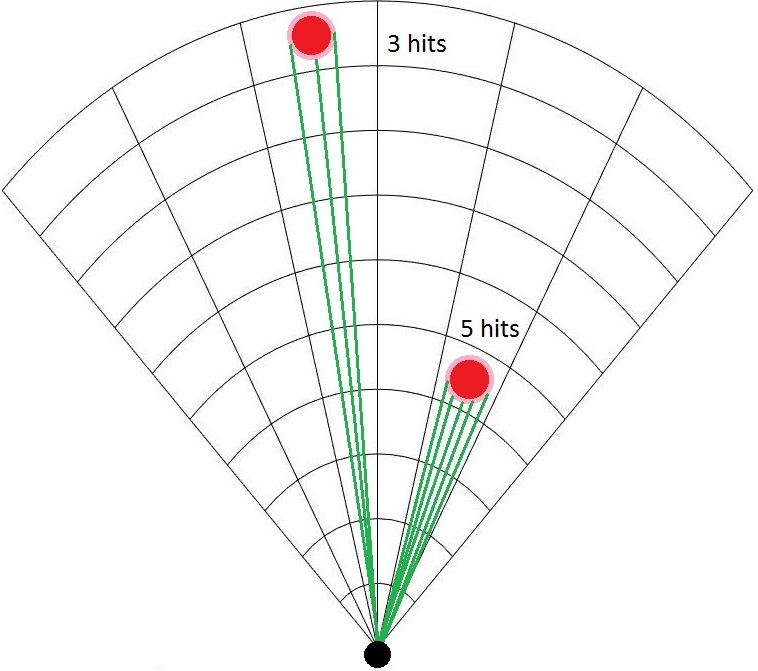
\includegraphics[width=0.7\textwidth]{\FIGDIR/TE051CountOfLiDARHits}
    \caption{Different count of LiDAR hits with different distance from UAS.}
    \label{fig:P01CountOfLiDARHits}
\end{figure}


\paragraph{Map and Detected Obstacles Fusion:} The concept of \emph{offline/online obstacle map} is mandatory in modern obstacle avoidance systems and increases the safety of navigation/avoidance path. The \emph{older} concept was considering only LiDAR reading or \emph{real-time sensor readings} in general \cite{gomola2017probabilistic}. 

\begin{figure}[htbp]
    \centering
    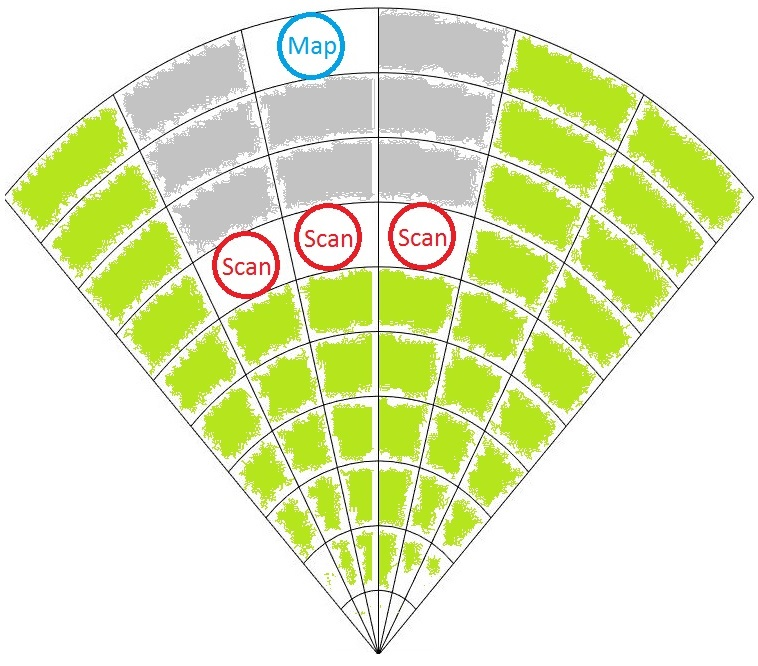
\includegraphics[width=0.7\textwidth]{\FIGDIR/TE053OvershadowedMapobstacle}
    \caption{Overshadowed map obstacle by detected obstacles.}
    \label{fig:P02OvershadowedMapobstacle}
\end{figure}

\newpage\noindent The fusion of real time sensor readings and obstacle map (prior knowledge) is required. Data fusion of these two sources is strongly depending on visibility property, because there are three basic scenarios:

\begin{enumerate}
    \item \emph{Dual detection} - the obstacle is marked on the map and detected by sensory system at some point of the time (older concept works).
    
    \item \emph{Hindered vision} - the detected obstacles are hindering vision to map obstacle therefore map obstacle uncertainty arises (older concept fails). 
    
    \item \emph{False-positive map} - map obstacle occupied space is visible by sensory system, but negative detection is returned. Therefore the map is giving \emph{false-positive} information.
\end{enumerate}

\noindent The second case is given in fig. \ref{fig:P02OvershadowedMapobstacle}, where map obstacle (blue circle) is overshadowed by three scanned obstacles (red circle). The visible space is denoted by green fill, the invisible space is denoted by gray fill. 
    	\subsection{(R) Detected obstacles}\label{s:detectedObstacles}
\paragraph{Idea:} The \emph{visibility} inside avoidance grid and \emph{obstacle} probability are interconnected for most ranging sensors (ex. LiDAR). The goal of this section is to introduce \emph{visibility hindrance} concept which includes space uncertainty assessment and detected obstacle  processing.

\paragraph{Detected Obstacle Rating:} The \emph{detected obstacle rating} defines UAS chances to encounter detected obstacle in avoidance grid $cell_{i,j,k}$. Final \emph{detected obstacle rating} is merged information (eq. \ref{eq:detectedObstacleRatingForCell}). The \emph{sensor field} can contain \emph{multiple} \emph{static obstacle sensors}.

\paragraph{Detected Obstacle Rate for LiDAR:},Lets have only one sensor set as homogeneous two axis rotary LiDAR. For one $cell_{i,j,k}$ there exists set of passing LiDAR beams:

\begin{equation}\label{eq:lidarRaysTroughCell}
    lidar Rays(cell_{i,j,k})=
    \left\{
        \begin{aligned}
        \left[
            \begin{gathered}
                horizontal^\circ\in horizontal Offsets,\\
                vertical^\circ\in vertical Offsets
            \end{gathered}
        \right]\in\R^2:&\\
        horizontal^\circ\in cell_{i,j,k}.horizontal &Range,\\
        vertical^\circ\in cell_{i,j,k}.vertical &Range\\
        \end{aligned}
    \right\}
\end{equation}

\noindent The horizontal and vertical offset of LiDAR ray is homogeneous. Meaning the horizontal/vertical distances between each two neighbouring LiDAR beams are equal.

The set $lidar Rays(cell_{i,j,k}))$ (eq. \ref{eq:lidarRaysTroughCell}) is finite countable and nonempty for any $c_{i,j,k}$, otherwise it will contradict   the definition of avoidance grid (def. \ref{def:AvoidanceGrid}).

The hit function $lidarScan()$ returns a distance of single beam return for beam with dislocation $[horizontal^\circ,$ $vertical^\circ]$ $\in$ $lidar Rays(cell_{i,j,k})$ angle offsets. The set of LiDAR hits (eq. \ref{eq:lidarHitFunction}) in cell $cell_{i,j,k}$ is defined like follow:

\begin{equation}\label{eq:lidarHitFunction}
    lidar Hits(cell_{i,j,k})=\left\{
        \begin{aligned}
        \left[
            \begin{gathered}
                distance=lidar Scan(),\\
                horizontal^\circ\in horizontal Offsets,\\
                vertical^\circ\in vertical Offsets
            \end{gathered}
        \right]\in\R^2:&\\
        distance \in cell_{i,j,k}.distance &Range,\\
        horizontal^\circ\in cell_{i,j,k}.horizontal &Range,\\
        vertical^\circ\in cell_{i,j,k}.vertical &Range\\
        \end{aligned}
    \right\}
\end{equation}

\noindent The \emph{naive} obstacle rate in case of LiDAR sensor defined as ratio between landed hits and possible hits:

\begin{equation}\label{eq:naiveObstacleRate}
    obstacle^{LiDAR}_{cell_{i,j,k}}=\frac{lidar Hits(cell_{i,j,k})}{lidar Rays(cell_{i,j,k})}
\end{equation}

\begin{note}
    The \emph{naive obstacle rate} (eq. \ref{eq:naiveObstacleRate}) ignores that \emph{LiDAR rays} are getting more far apart from each other. The \emph{cell surface} is increasing with cell distance from \emph{UAS}.
\end{note}

\noindent The hindrance (eq. \ref{eq:probabilityOfVisibilityHindrance}) rate is naturally defined as supplement to naive obstacle rate. This definition is sufficient, because its reflecting the \emph{remaining sensing capability} of  LiDAR.

\begin{equation}\label{eq:probabilityOfVisibilityHindrance}
    hindrance^{LiDAR}_{cell_{i,j,k}}=1-\frac{lidar Hits(cell_{i,j,k})}{lidar Rays(cell_{i,j,k})}
\end{equation}

\paragraph{Cell Density Function:}  Let`s start with differential form of cell surface (eq. \ref{eq:finalCellSquare}). The target object have several hits in \emph{Avoidance Grid}. Target $cell_{i,j,k}$ has following properties which are used in surface calculation:
\begin{enumerate}
    \item \textit{Horizontal span} - defines range of horizontal scanner partition.
    \item \textit{Vertical span} - defines range of vertical scanner partition.
\end{enumerate}

\noindent By rewriting (eq. \ref{eq:finalCellSquare}) and using horizontal range parameter and inverted vertical range parameter following surface integral is obtained (eq. \ref{eq:cellSurfaceIntengralDelta}).

\begin{multline}\label{eq:cellSurfaceIntengralDelta}
    Area(cell_{i,j,k}) =\\ \int_{horizontal_{start}^\circ}^{horizontal_{end}^\circ}\int_{vertical_{end}^\circ}^{vertical_{start}^\circ} radius^2 \cos(vertical^\circ) \quad \text{d} vertical^
    \circ\text{d} horizontal^\circ
\end{multline}

\begin{note}
    The \emph{radius} parameter is \emph{average} distance of hits landed in $cell_{i,j,k}$. This helps to reflect real \emph{scanned surface}.
\end{note}

Numerically stable integration exist for boundaries $horizontal^\circ \ in [-\pi,\pi]$, $vertical^\circ \in [-\frac{\pi}{2},\frac{\pi}{2}]$ given as follow:

\begin{multline}\label{eq:intersectionSurfaceForCell}
    Area(radius,horizontal Range, vertical_{start}^\circ, vertical_{end}^\circ) =\dots\\ 
    =\left\{
    \begin{aligned}
        vertical&_{start}^\circ <0, vertical_{end}^\circ \le 0 :\\ 
            &radius^2(\sin |vertical_{start}^\circ| - \sin|vertical_{end}^\circ|)\times horizontal Range)\\
         vertical&_{start}^\circ <0, vertical_{end}^\circ > 0   :\\
            & r^2(\sin |vertical_{start}^\circ| + \sin|vertical_{end}^\circ|)\times horizontal Range)\\
         vertical&_{start}^\circ \ge 0 vertical_{end}^\circ < 0 :\\
            & r^2(\sin vertical_{end}^\circ- \sin vertical_{start}^\circ)\times horizontal Range)
    \end{aligned}
    \right.
\end{multline}

\noindent An intersection surface for cell is defined in (eq. \ref{eq:intersectionSurfaceForCell}). Area covered by LiDAR hits (eq. \ref{eq:lidarHitArea}) is defined as LiDAR hit rate (hits to passing rays ratio) multiplied by \emph{Average} cell intersection surface (eq. \ref{eq:intersectionSurfaceForCell}).

\begin{equation}\label{eq:lidarHitArea}
    lidar Hit Area(cell_{i,j,k}) = \frac{lidar Hits(cell_{i,j,k})}{lidar Rays(cell_{i,j,k})} \times Area\left(\begin{gathered}radius,horizontal Range,\\ vertical_{start}^\circ, vertical_{end}^\circ\end{gathered}\right)
\end{equation}

\noindent There is user defined parameter for \emph{LiDAR treshold area}, which represents minimal considerable surface area for obstacle to be threat. The \emph{detected obstacle rate} considering surface is defined in (eq. \ref{eq:lidarHitFormula}) and it removes bias of naive approach (eq.\ref{eq:naiveObstacleRate}).

\begin{equation}\label{eq:lidarHitFormula}
    obstacle(LiDAR,cell_{i,j,k})=\min\left\{\frac{lidar Hit Area(cell_{i,j,k})}{UAS.lidar Threshold Area},1\right\}
\end{equation}



\paragraph{Visibility Rate for  LiDAR:} For each $cell_{i,j,k}$ and each sensor in sensor field there exist hindrance rate, which defines how much vision is clouded in single cell. Example of hindrance calculation for LiDAR has been given by (eq. \ref{eq:probabilityOfVisibilityHindrance}). Let us consider cell row $cell Row (j_{fix},$ $k_{fix})$ with fixed horizontal index $j_fix$ and vertical index $k_{fix}$ is given as series of cells (eq. \ref{eq:cellrowDefinition}).

\begin{equation}\label{eq:cellrowDefinition}
    cellRow(j_{fix},k_{fix})= \left\{cell_{i,j,k}\in Avoidance Grid :\begin{aligned}&i\in\{1,..,layersCount\},\\&j=j_{fix}, k=k_{fix}\end{aligned}\right\}
\end{equation}

For each $cell_{i,j,k}$ there exists a function which calculates final visibility hindrance rate. Then for ordered cell row:
\begin{equation*}
    cell Row(j_{fix},k_{fix}) = \{cell_{1,j_{fix},k_{fix}},  cell_{2,j_{fix},k_{fix}}, \dots, cell_{layers Count,j_{fix},k_{fix}}\}    
\end{equation*}
and for one selected $cell_{i,j,k}$ the visibility rate is naturally defined as a supplement to hindrance from previous cells. The visibility is defined in (eq. \ref{eq:FinalVisibilityProbability}).

\begin{multline}\label{eq:FinalVisibilityProbability}
    visibility(cell_{i_c,j_c,k_c})=\dots\\ \dots =1 - \sum_{index\in\N^+}^{index < i_c} hindrance(cell_{a,j_c,k_c}: cell_{a,j_c,k_c}\in cell Row(j_{c},k_{c})
\end{multline}

\paragraph{Example:} Let be $cell_{4,j_{fix},k_{fix}}$ is selected for visibility rate assessment, then $cell_{1,j_{fix},k_{fix}}$, $cell_{2,j_{fix},k_{fix}}$, and $cell_{3,j_{fix},k_{fix}}$, are used as a base of cumulative hindrance rate.

\noindent \emph{The cumulative hindrance rate} for any $cell Row(j_{fix},k_{fix})$ is bounded:

\begin{equation}
    0 \le \sum_{cell\in cell Row(j_{fix},k_{fix})} visibility(cell) \le 1
\end{equation}

\begin{note}
    A \emph{cumulative hindrance rate} does not always reach 1 in case of LiDAR sensor, because some rays may pass or hit after leaving \emph{avoidance grid} range.
\end{note}


\begin{figure}[H]
    \centering
    \begin{subfigure}{0.32\textwidth}
        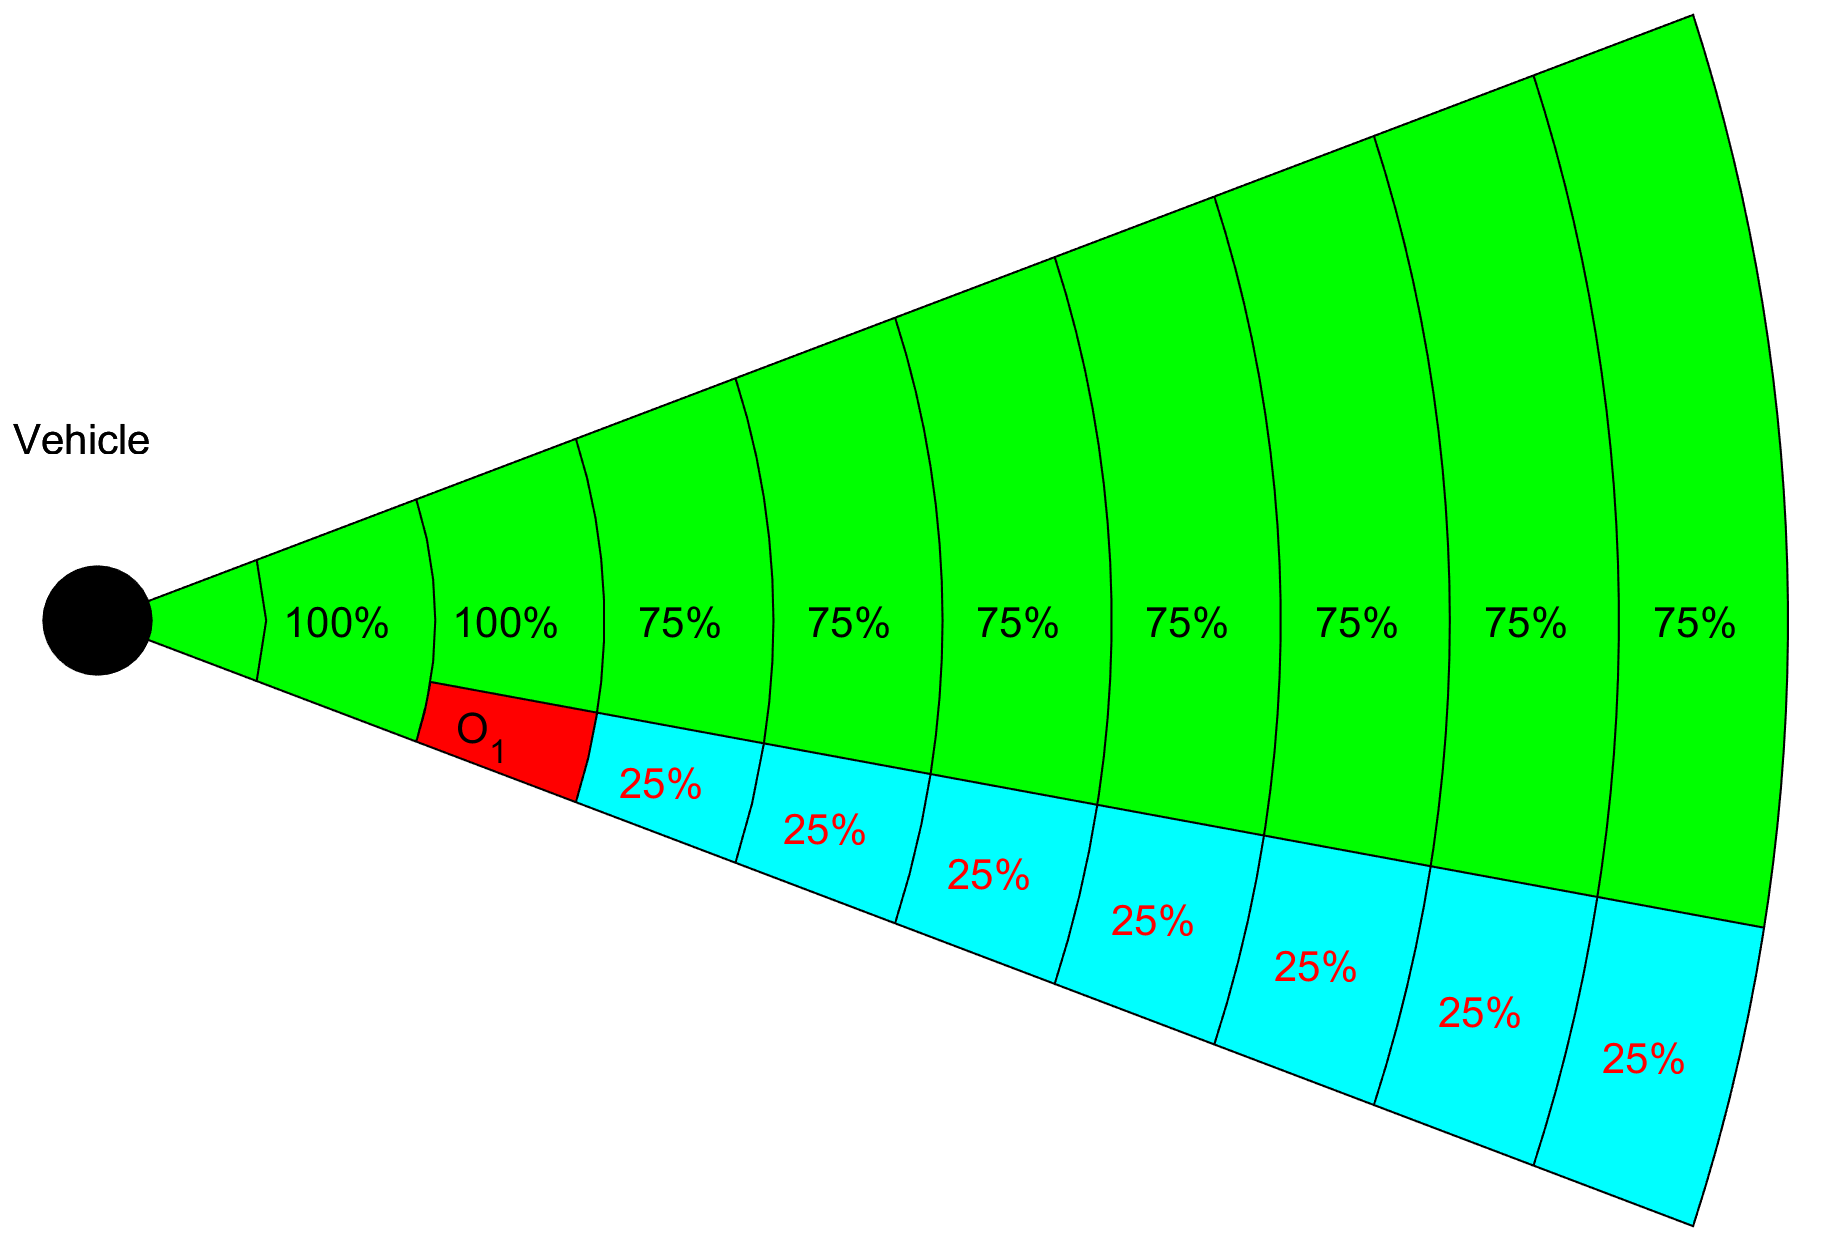
\includegraphics[width=0.9\linewidth]{\FIGDIR/TE006VisibilityFirstObstacle} 
        \caption{1\textsuperscript{st} hindrance.}
        \label{fig:fistObstacleHindrance}
    \end{subfigure}
    \begin{subfigure}{0.32\textwidth}
        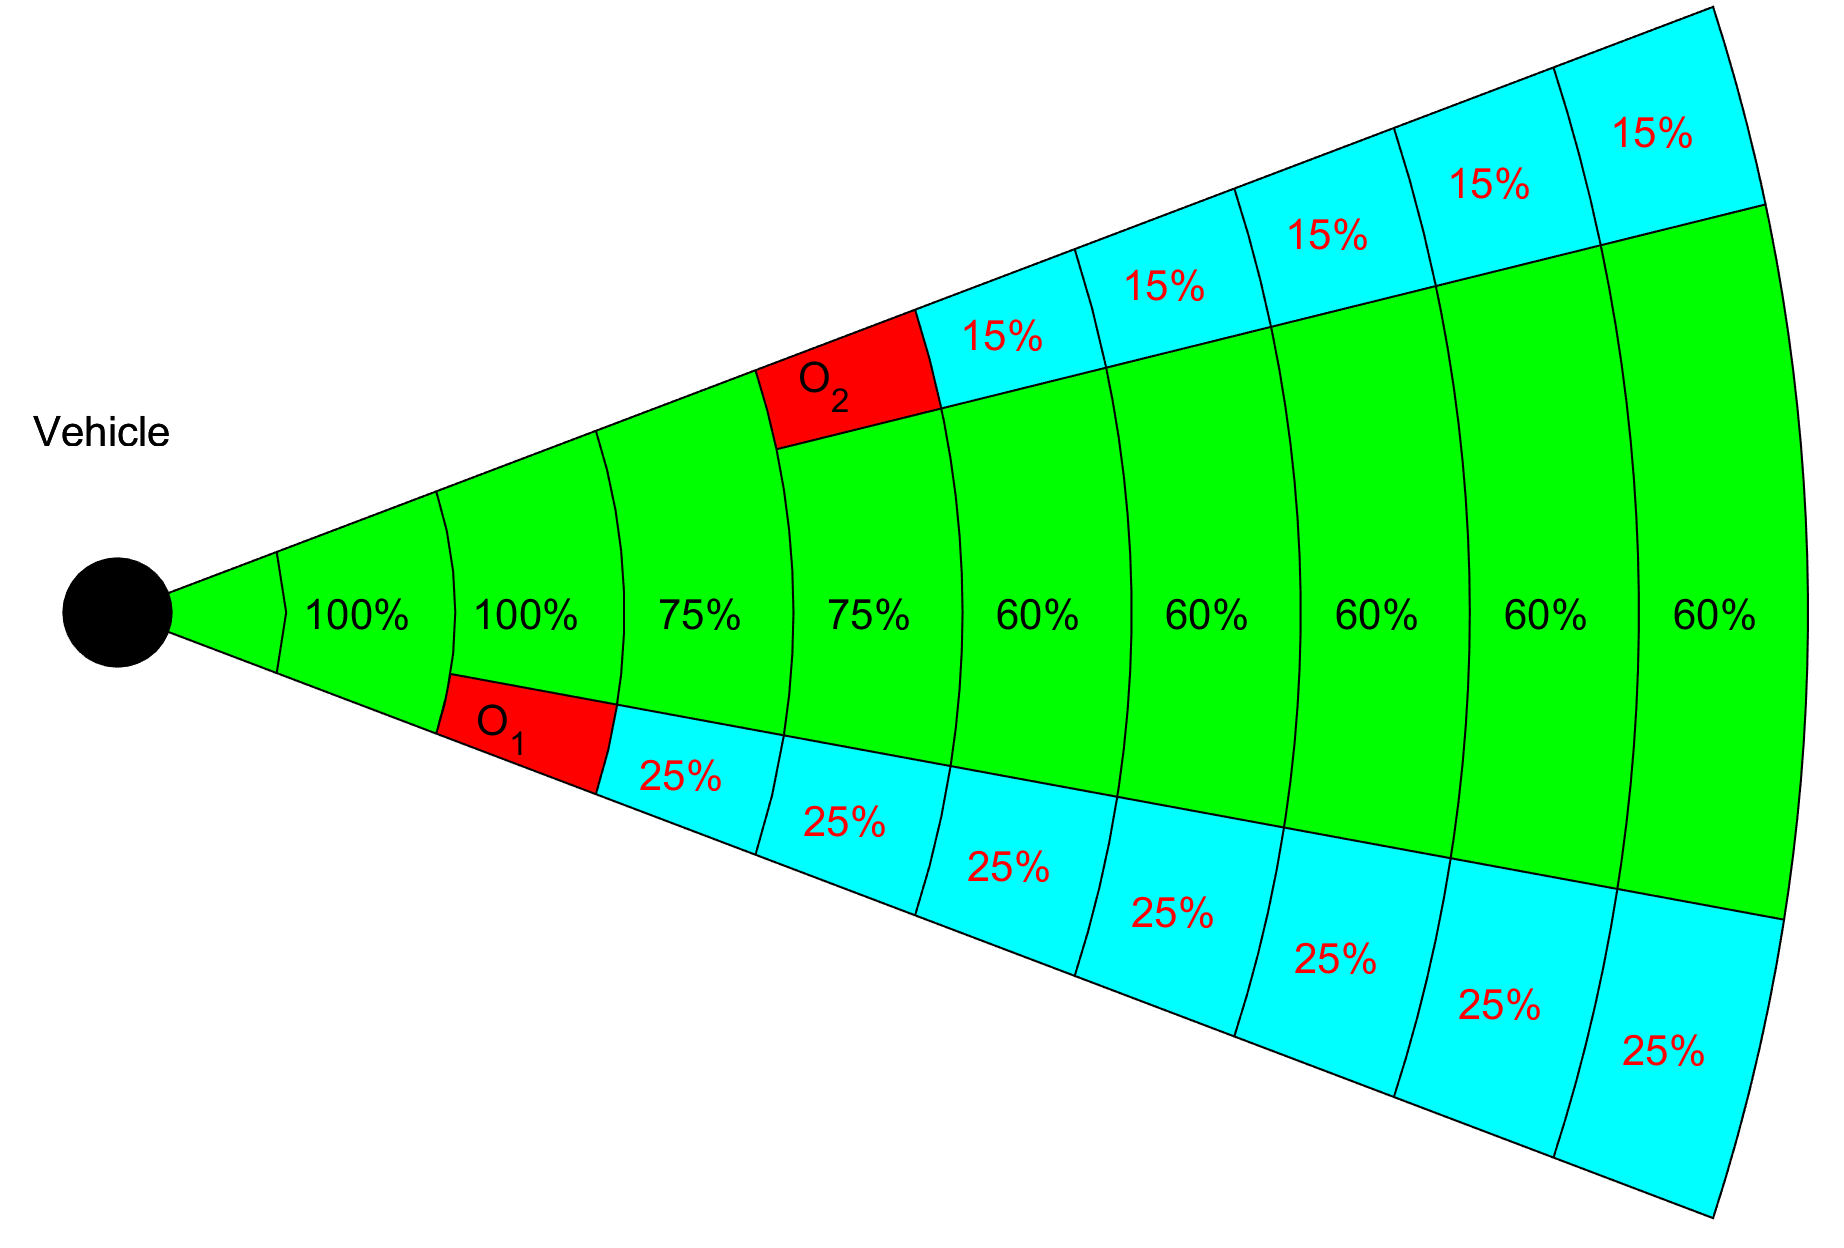
\includegraphics[width=0.9\linewidth]{\FIGDIR/TE007VisibilitySecondObstacle} 
        \caption{2\textsuperscript{nd} hindrance.}
        \label{fig:secondObstacleHindrance}
    \end{subfigure}
    \begin{subfigure}{0.32\textwidth}
        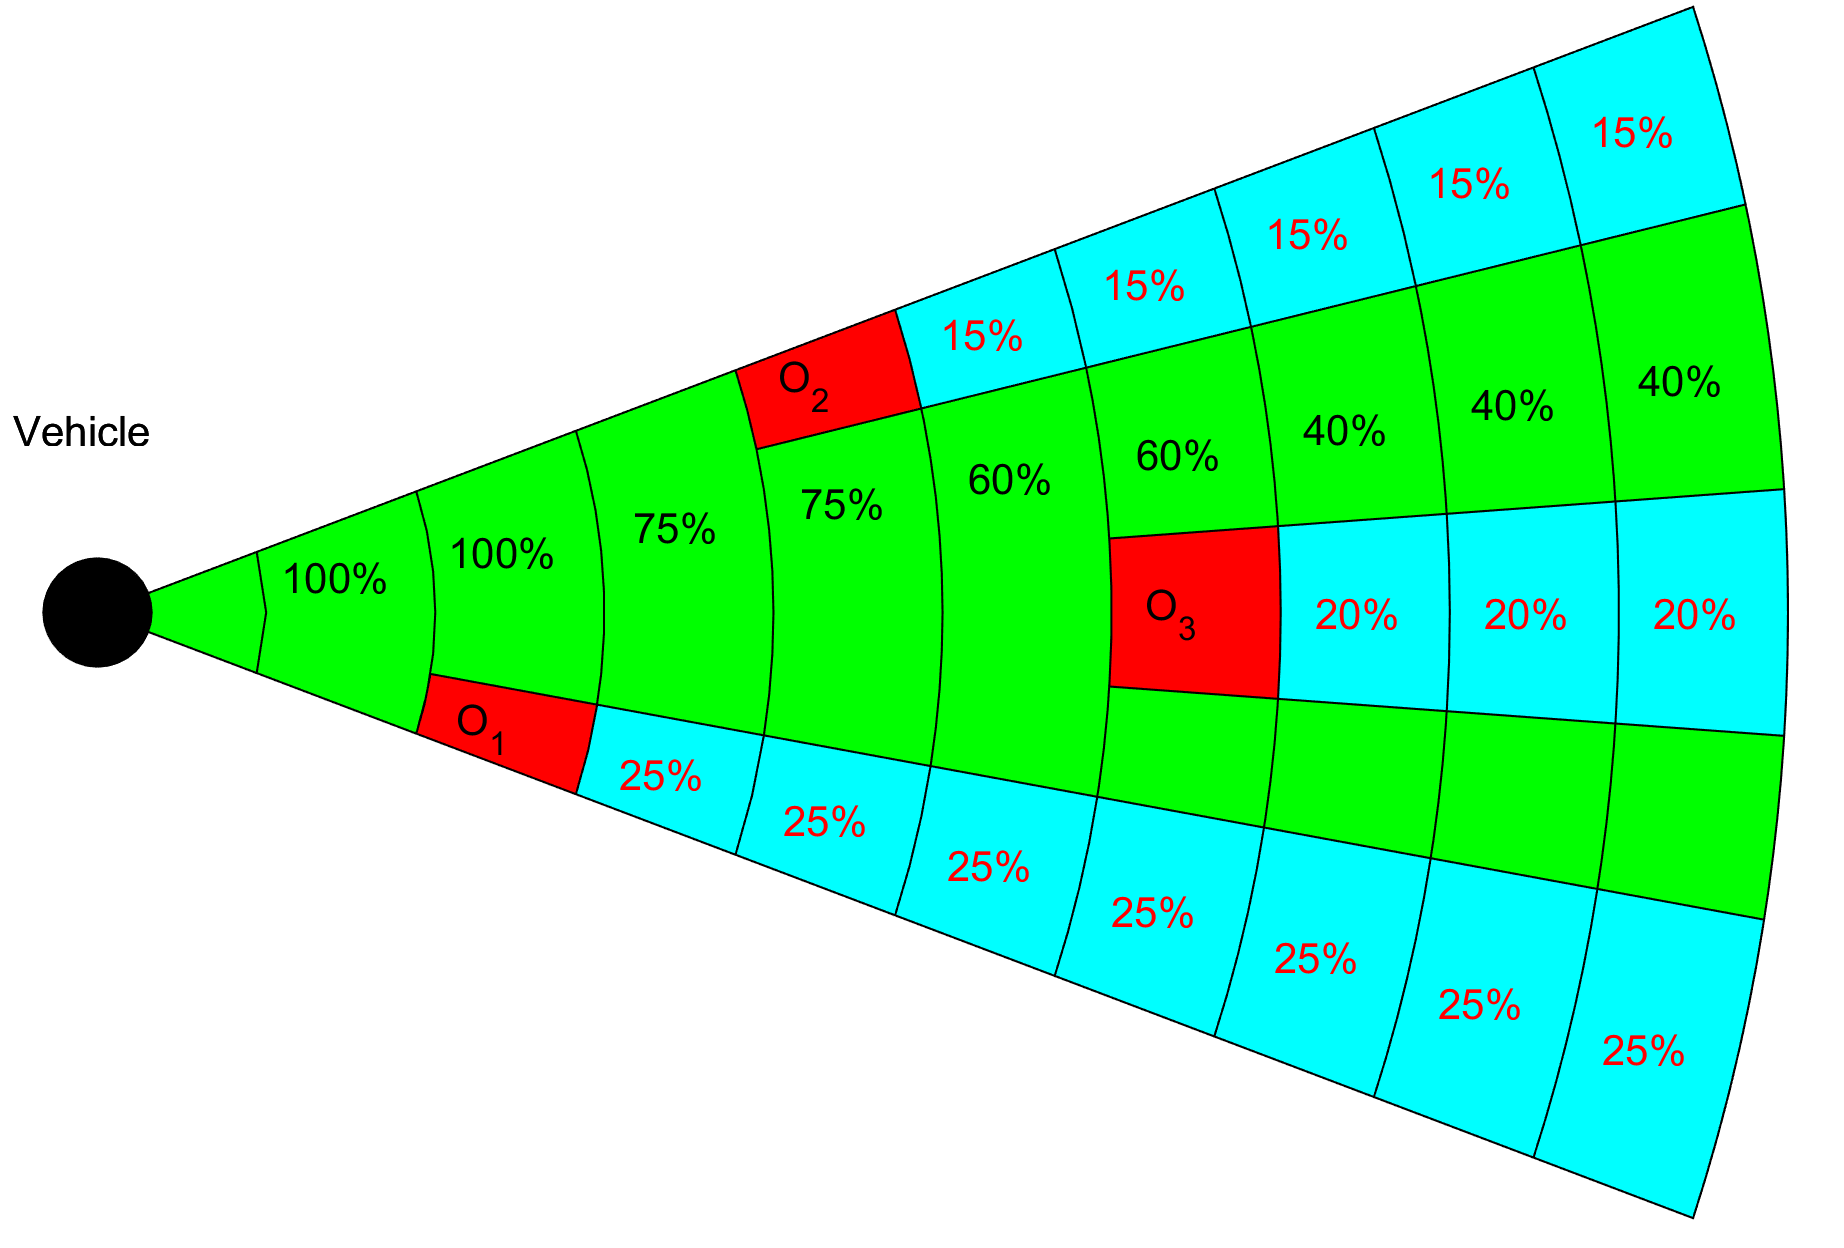
\includegraphics[width=0.9\linewidth]{\FIGDIR/TE008VisibilityThirdObstacle} 
        \caption{3\textsuperscript{rd} hindrance.}
        \label{fig:thirdObstacleHindrance}
    \end{subfigure}
    \caption{Obstacle hindrance impact on visibility in \emph{Avoidance Grid Slice}.}
    \label{fig:hindranceImpactOnVisibility}
\end{figure}

For one cell row $cell Row(j_{fix},k_{fix})$, where count of layers is equal to 10, and layers have equal spacing. There is LiDAR sensor

During consequent LiDAR scans $s(t_0)$, $s(t_1)$, $s(t_2)$, and $s(t_3)$ the obstacle sets $\mathscr{O}_1(t_1)=\{o_1\}$, $\mathscr{O}_2(t_2)=\{o_1,o_2\}$, and $\mathscr{O}_3(t_3)=\{o_1,o_2,o_3\}$ are discovered. Assigned hindrance rates are like follow:

\begin{enumerate}
    \item\emph{Time $t_0$} - there is no obstacle nor hindrance, all cells are fully visible.

    \item\emph{Time $t_1$} (fig. \ref{fig:fistObstacleHindrance}) - $\mathscr{O}_1(t_1)=\{o_1\}$ was detected, the hindrance rate  for $cell_{3,j_{fix},k_{fix}})$ is equal to $0.25$. The visibility rate in cells $cells_{4-10,j_{fix},k_{fix}}$ is $0.75$. 
    
    \item\emph{Time $t_2$} (fig. \ref{fig:secondObstacleHindrance}) - $\mathscr{O}_2(t_2)=\{o_1,o_2\}$ was detected, the additional hindrance rate for $cell_{5,j_{fix},k_{fix}}$ is $0.15$. The visibility rate in  $cells_{6-10,j_{fix},k_{fix}}$ is lowered by additional $0.15$ and its set to $0.60$ now.
    
    \item\emph{Time $t_3$} (fig. \ref{fig:thirdObstacleHindrance}) - $\mathscr{O}_3(t_3)=\{o_1,o_2,o_3\}$  was detected the additional hindrance rate for  $cell_{7,j_{fix},k_{fix}}$ is $0.20$. The visibility rate in $cells_{8-10,j_{fix},k_{fix}}$ is lowered by additional $0.20$ and its set to $0.40$  now.
\end{enumerate}
		%\subsection{\secState{R}Map Obstacles}\label{s:mapObstacles}
\paragraph{Map Obstacles:} Use \emph{stored LiDAR readings} from previous mission to build an compact obstacle map \cite{cernamaria2018}. Then use \emph{this map} as a additional information source.

\begin{figure}[H]
    \begin{subfigure}{0.32\textwidth}
        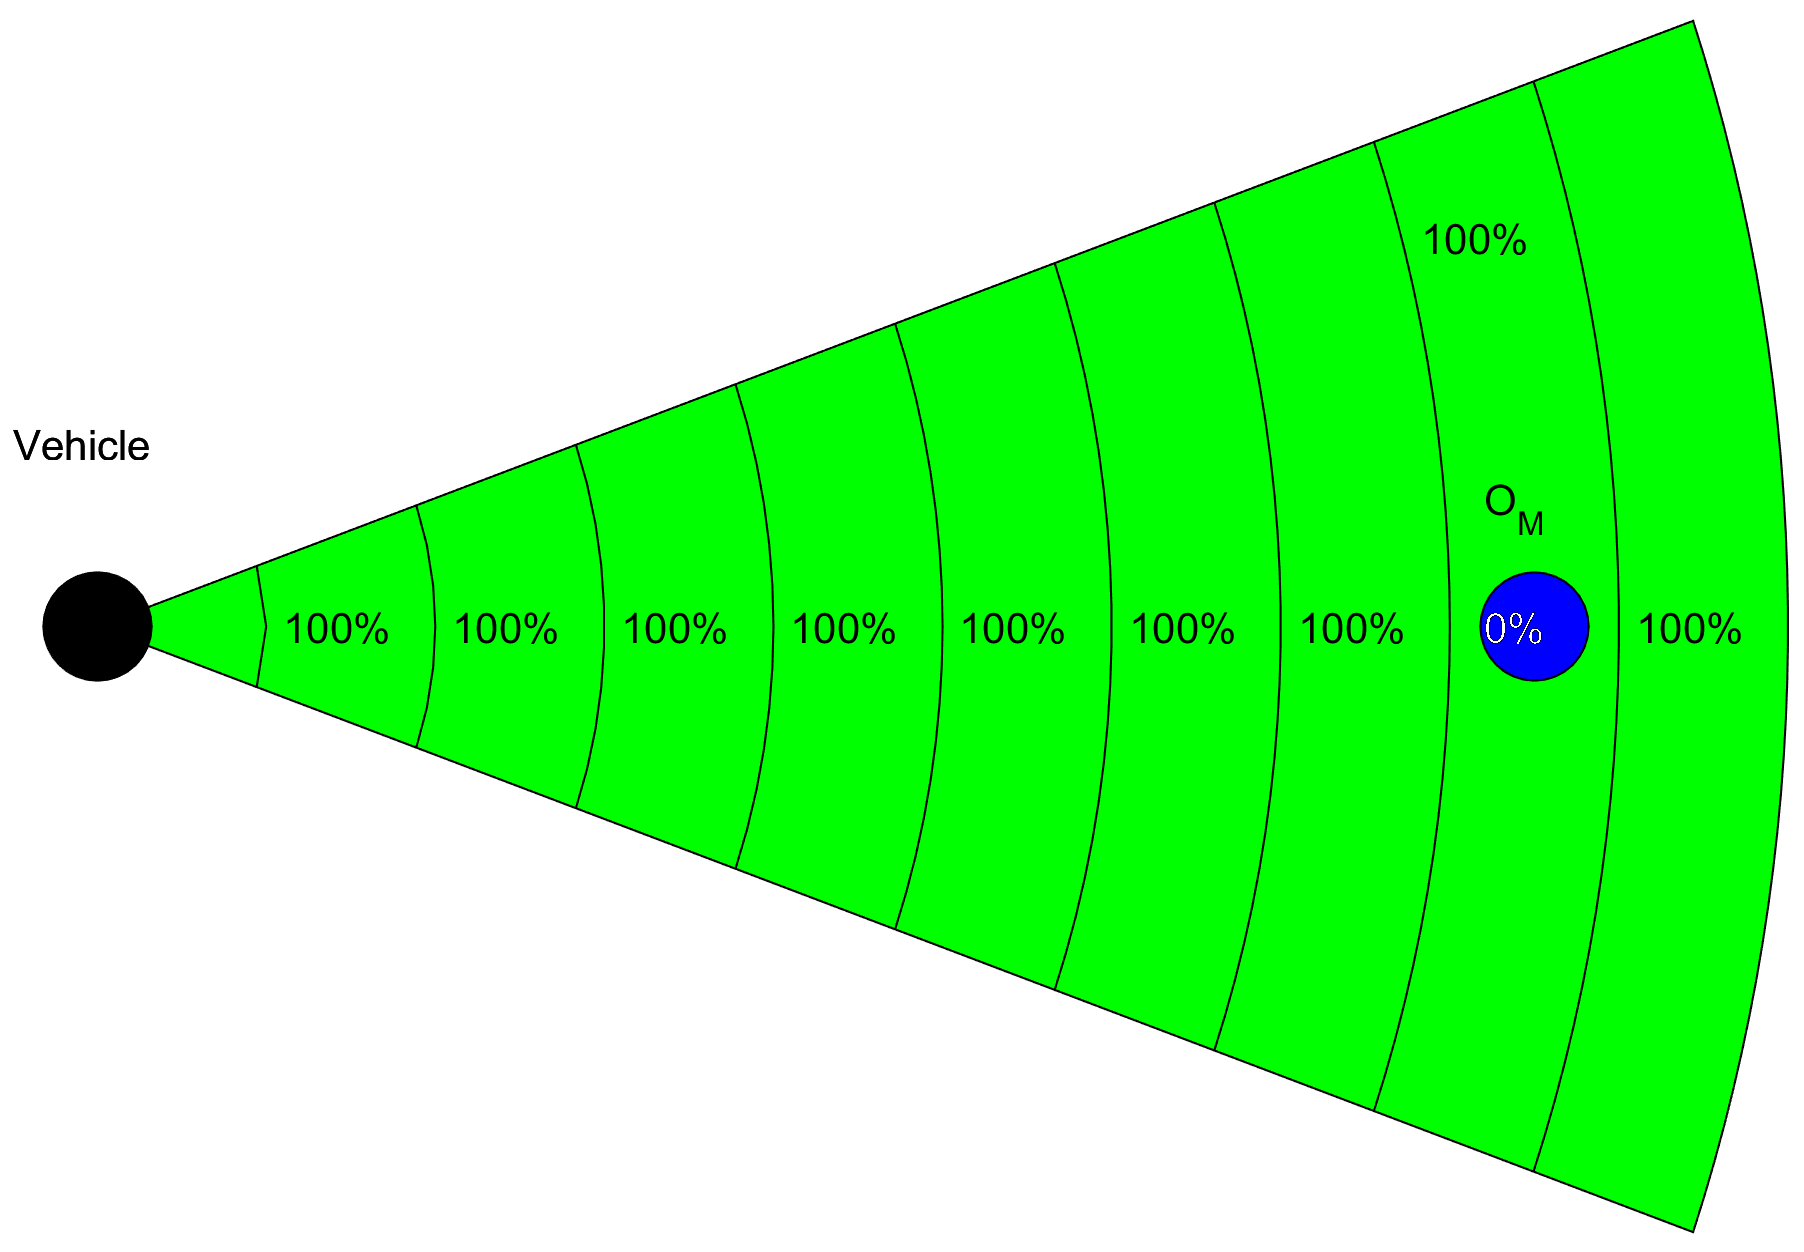
\includegraphics[width=0.9\linewidth]{\FIGDIR/TE009MapObstacleUndetected} 
        \caption{Undetected.}
        \label{fig:undetectedMapObstalce}
    \end{subfigure}
    \begin{subfigure}{0.32\textwidth}
        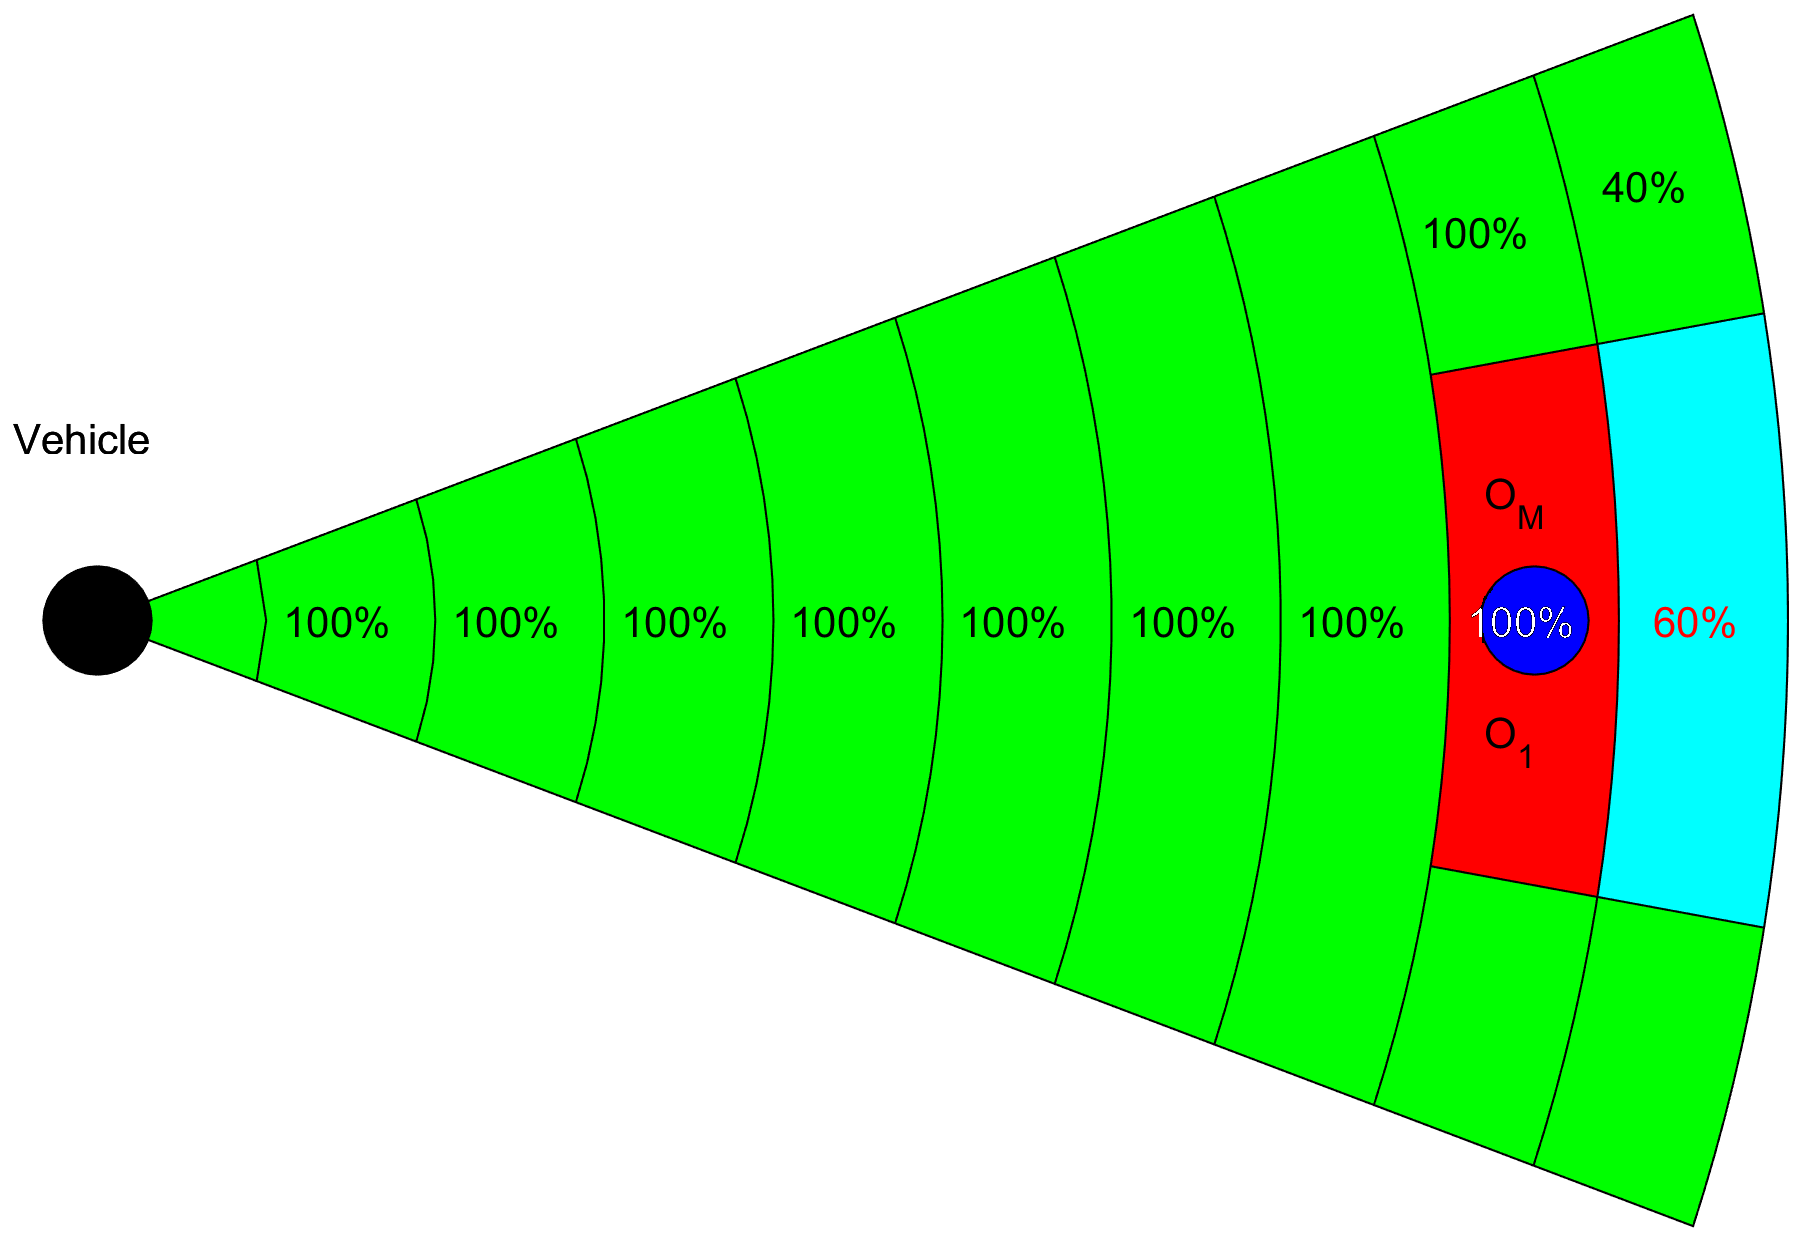
\includegraphics[width=0.9\linewidth]{\FIGDIR/TE010MapObstacleDetected} 
        \caption{Detected.}
        \label{fig:detectedMapObstacle}
    \end{subfigure}
    \begin{subfigure}{0.32\textwidth}
        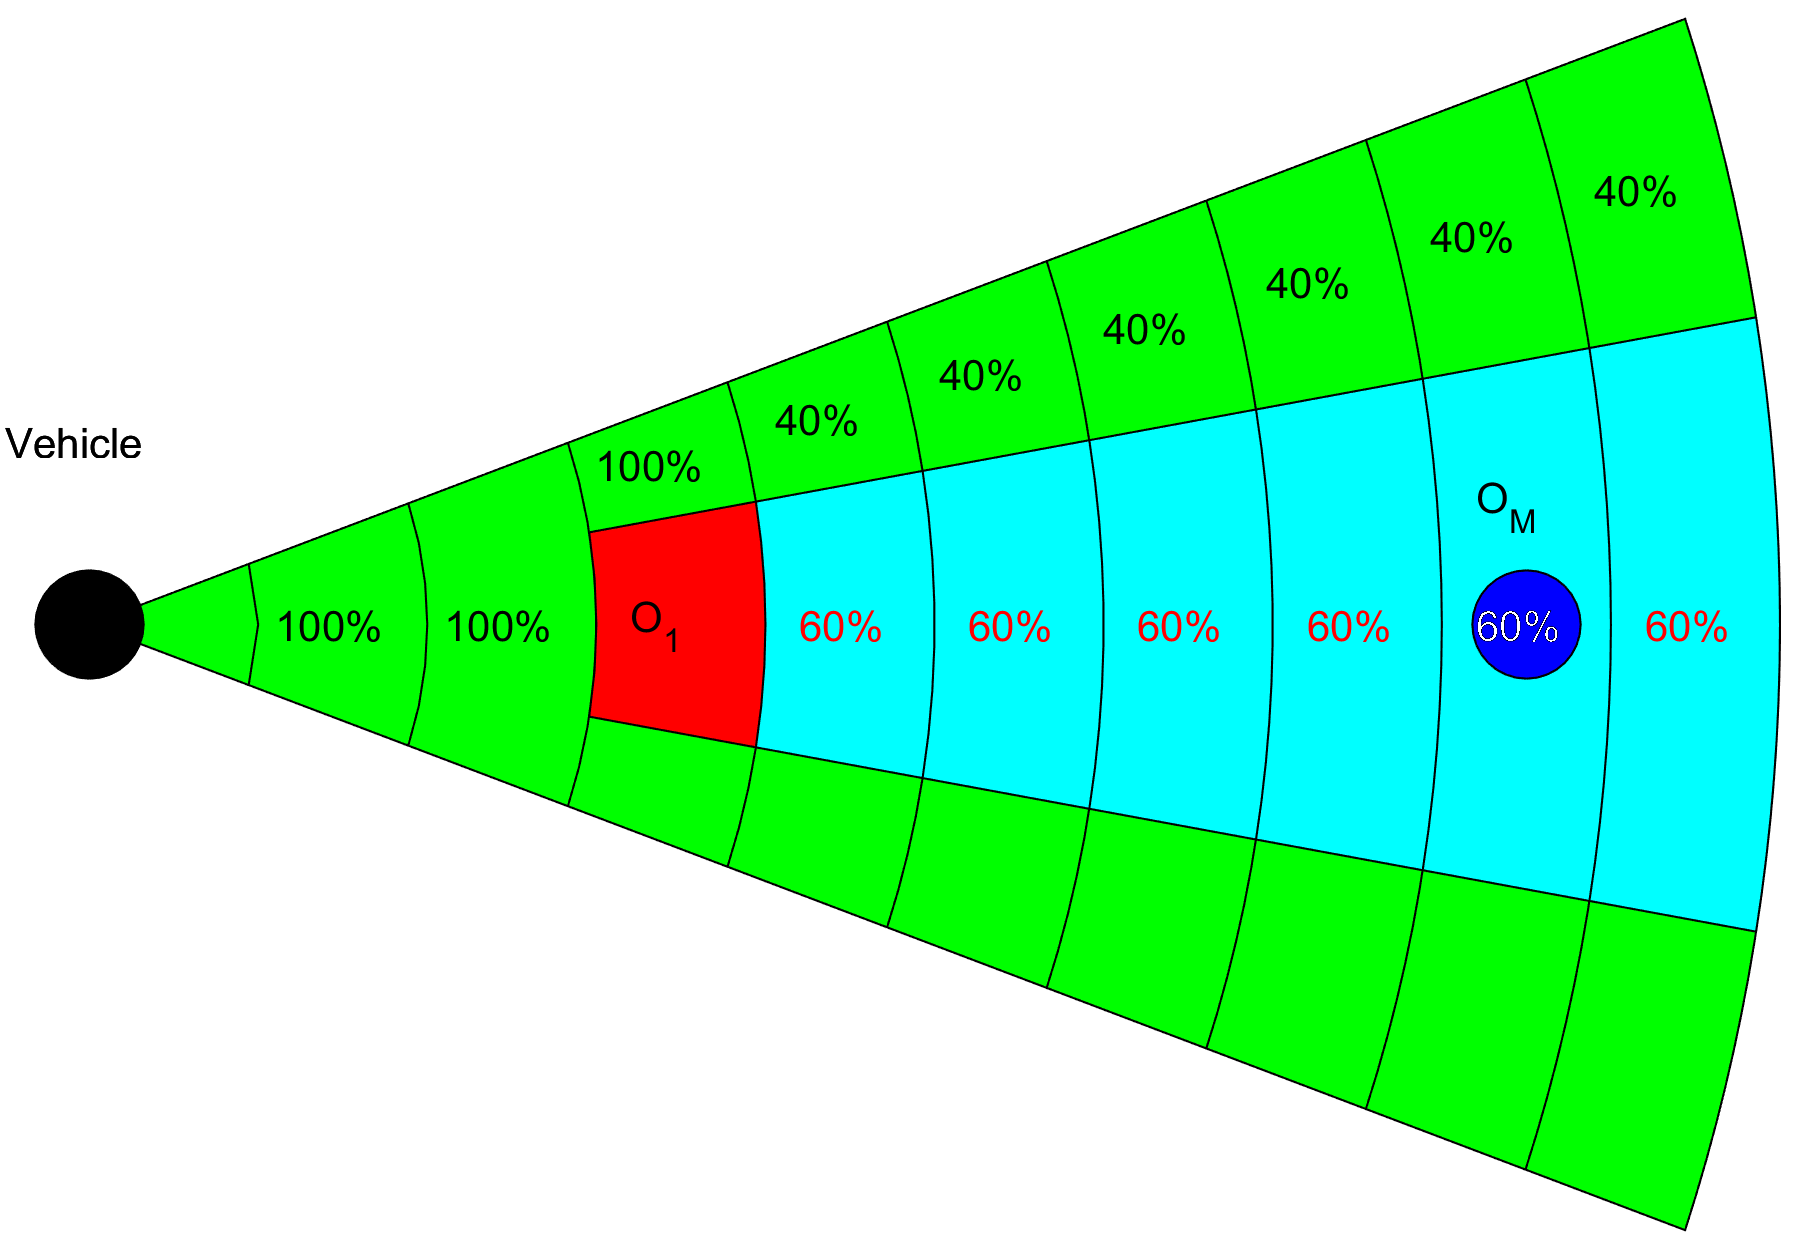
\includegraphics[width=0.9\linewidth]{\FIGDIR/TE011MapObstacleHiden}
        \caption{Hindered.}
        \label{fig:hinderedMapObstacle}
    \end{subfigure}
    \caption{Map obstacle states after \emph{Data fusion}.}
    \label{fig:mapObstacleStatesAfterDataFusion}
\end{figure}

\paragraph{Concept:} A \emph{map obstacle} state has very simple logic, there are three possible cases:

\begin{enumerate}
    \item \emph{Undetected} - Map obstacle $O_M$ is charted on map (fig. \ref{fig:undetectedMapObstalce}), but is undetected by any sensor in sensor field, therefore the probability of map obstacle occurrence is equal to $0$.


    \item \emph{Detected} Map obstacle $O_M$ is charted on map and detected by any sensor in sensor field (fig. \ref{fig:detectedMapObstacle}). The map obstacle rate is equal to detected obstacle rate, usually its equal to $1$.

    \item \emph{Hindered} Map obstacle $O_M$ is hindered behind other detected obstacle $O_1$ (fig. \ref{fig:hinderedMapObstacle}). The detected obstacle $O_1$ is in $cell_{i,j,k}$ and is reducing visibility in follow up $cellRow_{i_f>i,j,k}$ by $60$ percent.
\end{enumerate}

\paragraph{Implementation:} The formulation of final map obstacle rate  $map(cell_{i,j,k})$ was outlined in previous examples. These examples are showing the \emph{desired behaviour} and its solved by \emph{data fusion} (sec. \ref{s:sensorFusion}).

First we start with obstacle map definition. The obstacle map  (eq. \ref{eq:obstacleMap}) defines an map obstacle set of information vectors with position in global coordinate frame , orientation bounded to global coordinate reference frame, safety margin and additional parameters.
\begin{equation}\label{eq:obstacleMap}
    obstacle Map= 
    \left\{
    \begin{bmatrix}
        position,\\
        orientation,\\
        safety Margin,\\
        parameters
    \end{bmatrix}
    :
    \begin{aligned}
        & position \in  \R^3(GCF),\\
        & orientation \in \R^3(GCF),\\
        & safety Margin \in \R^+(m),\\
        & parameters \in \{\dots\}
    \end{aligned}
    \right\}
\end{equation}


The \emph{Map Obstacle} concept is taken from my \emph{master student work} \cite{cernamaria2018}, implementing \emph{compact representation} of point-cloud obstacle map. Te example of \emph{cuboid obstacles} with \emph{safe zone} is given in (fig. \ref{fig:exampleExtractedMapObstacles}).
    
\begin{figure}[H]
    \centering
    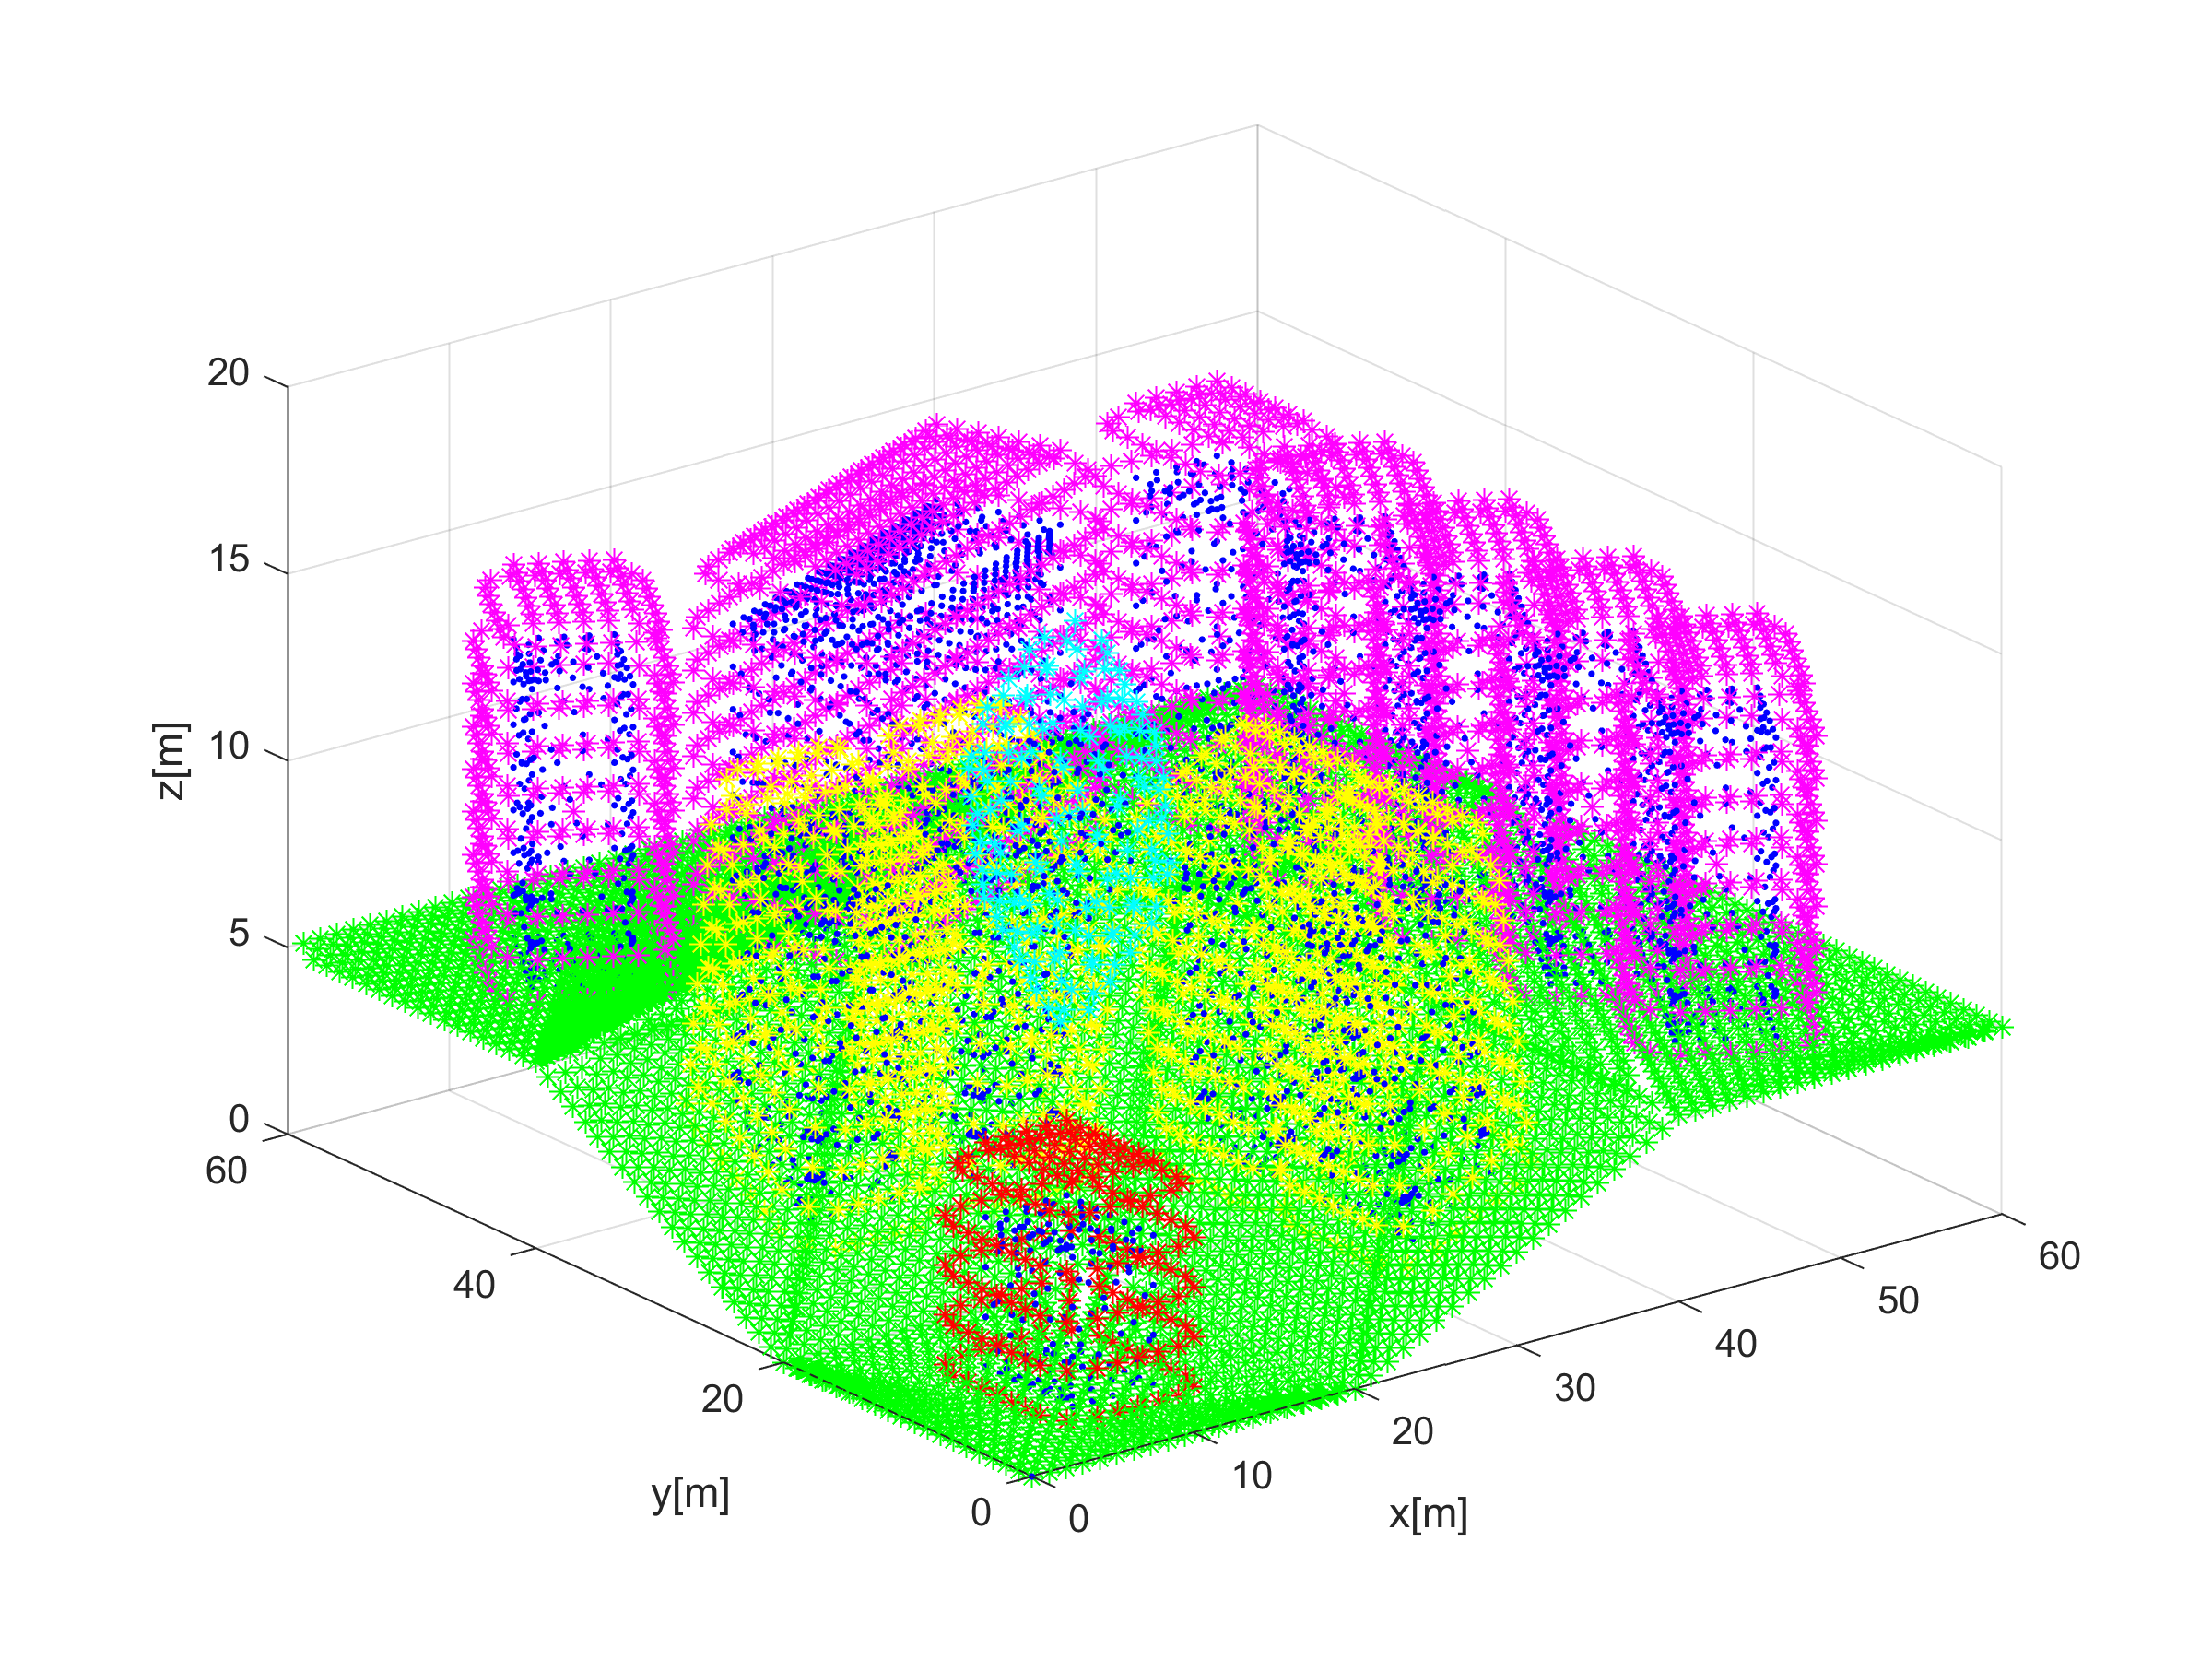
\includegraphics[width=0.7\textwidth]{\FIGDIR/TE054ExtractedMapObstaclesExample}
    \caption{Example of Extracted Map Obstacle \cite{cernamaria2018}.}
    \label{fig:exampleExtractedMapObstacles}
\end{figure} 

\noindent The space covered by any obstacle  is non-empty by definition. There are following types of map charted obstacles which are implemented in framework:

\begin{enumerate}
    \item\emph{Ball obstacle $parameters=\varnothing$} - simple ball with center at $position$, with offset safety margin.
    
    \item\emph{Line obstacle $parameters=[length]$} - simple line bounded by length $\in]0,\infty[$ with center at $position$ and given orientation with respect to main axis in global coordinate frame, with safety margin $<$ 0.
    
    \item\emph{Plane obstacle $parameters=[length,width]$} - bounded rectangle plane partition defined by length $\in]0,\infty[$, and width $w\in]0,\infty[$ with center at $\vec{p}$ and given orientation $\vec{o}$ with respect to main axis in global coordinate frame, with safety margin.
    
    \item\emph{Cuboid obstacle $parameters=[length,width,depth]$} - bounded cuboid space partition defined by length $\in]0,\infty[$, width $\in]0,\infty[$, and depth $d\in]0,\infty[$ with center at $position$ and rotated in orientation with respect to main axis in global coordinate frame, with safety margin.
\end{enumerate}

\noindent The \emph{map obstacles} are stored in clustered database. The \emph{selection criterion} is given in (eq. \ref{eq:mapObstacleSelectionCriterion}).

\begin{equation}\label{eq:mapObstacleSelectionCriterion}
    avoidance Grid.radius \ge distance(UAS.position,map Obstacle) - total Margin
\end{equation}

\noindent The \emph{total margin} is combination of \emph{safety margin} and \emph{body margin} (in case of line, plane, cuboid obstacle). The \emph{selection} was implemented as standard cluster select, selecting 26  surrounding clusters around UAS + own UAS cluster.

\noindent The \emph{compact obstacle representation} is transformed into \emph homogeneous point-cloud representations:

\begin{itemize}
    \item[1.]\emph{Body Point-cloud} - representing obstacle body approximation by geometrical shape (eq. \ref{eq:mapBodyPointCloud}). This point cloud is considered as hard constraints.
    
    \begin{equation}\label{eq:mapBodyPointCloud}
        body Point Cloud  =\{point\in\R^3(GCF): point \in map Obstacle Body\}
    \end{equation}
    
    \item[2.]\emph{Safety Margin Point Cloud} - representing safety coating around mapped obstacle body approximation (eq. \ref{eq:mapMarginPointCloud}). This point cloud is considered as soft constraint.
    \begin{equation}\label{eq:mapMarginPointCloud}
        margin Point Cloud = \{point\in\R^3(GCF): point \in map Safety Margin\}
    \end{equation}
\end{itemize}

\begin{note}
    The \emph{safety margin point cloud} is hollow in relationship to an \emph{body point cloud}, therefore:
    \begin{equation*}
        body Point Cloud \cap margin Point Cloud  = \varnothing
    \end{equation*}
\end{note}

\noindent The \emph{map obstacle} discretization to point cloud leads to problem how to calculate \emph{impact rate}. The \emph{theoretical impact rate} for \emph{obstacle} is given as:
\begin{equation*}
    impact Rate = \frac{volume(map Obstacle\cap cell_{i,j,k})}{volume(cell_{i,j,k})}\in [0,1]
\end{equation*}

\noindent The \emph{map obstacle related point clouds} (eq. \ref{eq:mapBodyPointCloud}, \ref{eq:mapMarginPointCloud}) are homogeneous \cite{cernamaria2018}. That means \emph{each point} in point clouds covers similar portion of object volume. There is \emph{threshold volume} (eq. \ref{eq:tresholdVolumeDefinition}) which represents minimal object volume to be considered as an \emph{obstacle}.

\begin{equation}\label{eq:tresholdVolumeDefinition}
    0< threshold Volume \le \frac{volume(point Cloud)}{|point Cloud|}
\end{equation}

\noindent The \emph{impact rate} of one point  when intersecting a $cell_{i,j,k}$ is given as count of \emph{threshold obstacle bodies} in \emph{point cloud covered mass} multiplied by inverted point count (eq. \ref{eq:pointImpactRateMap}).

\begin{equation}\label{eq:pointImpactRateMap}
    point. rate = \frac{point Cloud Volume}{threshold Volume}\times\frac{1}{|point Cloud|}
\end{equation}

The \emph{intersection set} between \emph{point cloud} and $cell_{i,j,k}$ is defined in (eq. \ref{eq:pointImpactRateMap}). The \emph{cell} intersection with points is defined in (eq. \ref{eq:boundedSpaceCell}).

\begin{multline}\label{eq:pointcloudIntersectionMap}
    intersection(map,cell_{i,j,k}) =\dots\\\dots \{points \in \R^3: (point\to Avoidance Grid Frame) \in cell_{i,j,k}\}
\end{multline}

\newpage \noindent The \emph{map obstacle rating} for $cell_{i,j,k}$ and obstacle for our \emph{information source} is defined in (eq. \ref{eq:mapcellratingourMap}).

\begin{equation}\label{eq:mapcellratingourMap}
    map(cell_{i,j,k},obstacle) =\max\left\{ \sum_{\forall point\in intersection(map,cell_{i,j,k})}  point.rate , 1\right\}
\end{equation}

\noindent The \emph{map obstacle rating} for $cell_{i,j,k}$ and \emph{our information source} is given as maximum of all possible cumulative ratings form each obstacle in \emph{active map obstacles} set (eq. \ref{eq:cumulativeMapCellRatingMap}).

\begin{equation}\label{eq:cumulativeMapCellRatingMap}
    map(cell_{i,j,k} = \max \left\{map(cell_{i,j,k},obstacle):\forall obstacle \in Active Map Obstacles\right\}
\end{equation}

\begin{note}
    The \emph{body point clouds} (eq. \ref{eq:mapBodyPointCloud}) never intersects, because they are created for inclusive obstacles. The \emph{safety margin point clouds} (eq. \ref{eq:mapMarginPointCloud}) can intersects, because they represents protection zones around physical obstacles. Therefore the \emph{maximum obstacle rating} (eq. \ref{eq:cumulativeMapCellRatingMap}) needs to be selected.
\end{note}

	    %Intruders
    	\subsection{Intruders}\label{s:intruders}
\paragraph{Intruder behavior:} \emph{Adversarial behavior} of moving obstacle is trying to destroy avoiding our UAS.  The \emph{Intruder} UAS \cite{fiorini1998motion} is not trying to hurt our \emph{UAS} actively. The \emph{Adversarial behaviour} is neglected in this work. The non-cooperative avoidance is assumed, it can be relaxed to \emph{cooperative avoidance} in \emph{UTM controlled airspace}.

\paragraph{Intruder information:} The \emph{observable intruder information set} for any kind of intruder, obtained through the sensor/C2 line, is following:
\begin{enumerate}
    \item\emph{Position} - position of an intruder in the \emph{local} or \emph{global} coordinate frame, which can be transformed into \emph{avoidance grid coordinate frame}.
    
    \item\emph{Heading and Velocity} - intruder heading and linear velocity in avoidance grid coordinate frame.
    
    \item\emph{Horizontal/Vertical Maneuver Uncertainty Spreads} - how much can an \emph{intruder} deviate from the \emph{original linear path} in a \emph{horizontal/vertical} plane in \emph{Global coordinate Frame}.
\end{enumerate}

 

\begin{figure}[H]
    \centering
    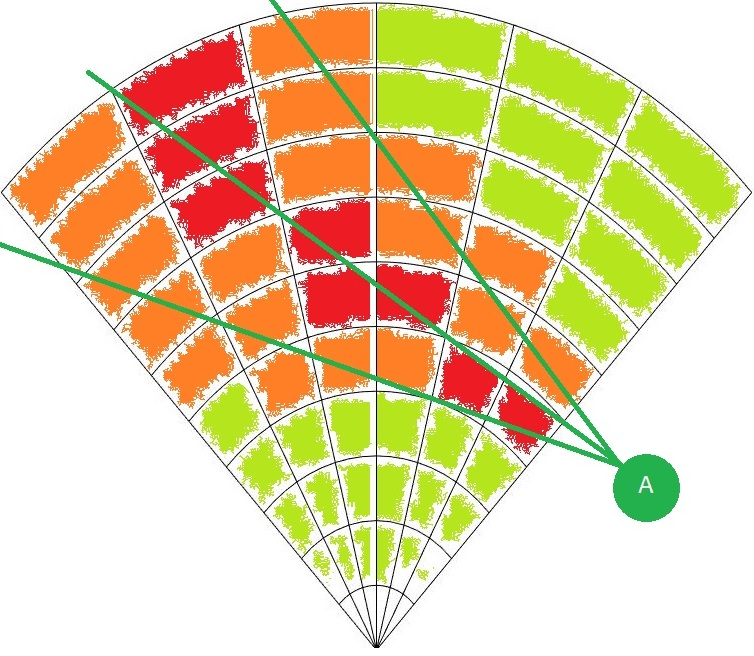
\includegraphics[width=0.7\textwidth]{\FIGDIR/TE052AdversaryProbabilitySpread}
    \caption{Intruder UAS intersection rate along the expected trajectory.}
    \label{fig:intruderProbabiltySpreadTheoretical}
\end{figure}   

\paragraph{Example of Intruder Intersection:} Let us neglect the \emph{time-impact} aspect on the \emph{intersection}.  The \emph{intruder} (black "I" circle) is intersecting one \emph{avoidance grid horizontal slice} (fig. \ref{fig:intruderProbabiltySpreadTheoretical}).  The intruder is moving along linear path approximation based on velocity (middle green line). The \emph{Horizontal Maneuver Uncertainty spread} is in \emph{green line boundary area} \emph{intruder intersection rating} is denoted as green-orange-red cell fill reflecting intersection severity:  red is a high rate of the intersection, orange is the medium rate of the intersection and green is a low rate of the intersection.
    


\paragraph{Moving Threats:} The \emph{UAS} can encounter following threats during the \emph{mission execution}:
\begin{enumerate}
    \item \emph{Non-cooperative Intruders} - the intruders who does not implement any approach to ensure mutual avoidance efficiency.
    
    \item \emph{Cooperative Intruders} - the intruders whom actively communicate or follow common agreed behavior pattern (ex. Rules of the Air).
    
    \item \emph{Moving Constraints} - the constrained portion of \emph{free} space which is shifting its boundary over time (ex. Short term bad weather).
\end{enumerate}
    
\begin{note}
    Our approach considers only \emph{UAS} intruders because \emph{Data Fusion} considers data received through \emph{ADS-B} messages. The \emph{Intruders} extracted from \emph{LiDAR} scan were not considered (ex. birds). The proposed \emph{intruder intersection models} are reusable for other \emph{intruder sources}.
\end{note}

\paragraph{Approach Overview:} The \emph{Avoidance Grid} (def. \ref{def:AvoidanceGrid}) is adapted to the \emph{LiDAR} sensor. The \emph{Euclidean grid intersections} are fairly simple. The \emph{polar coordinates grid} is not. The need to keep \emph{polar coordinates grid} is prevalent, because of fast \emph{LiDAR} reading assessment.  There are following commonly known methods to address this issue:

\begin{enumerate}
    \item\emph{Point-cloud Intersections} - the \emph{threat impact area} is discredited into a sufficiently thick point cloud. This point-cloud have \emph{point impact rate} and \emph{intersection time} assigned to each point. The \emph{point-cloud} is projected to \emph{Avoidance Grid}. If the \emph{impact point} hits $cell_{i,j,k}$ the cell`s impact rate is increased by the amount of \emph{point impact rate}. The final \emph{threat impact rate} in $cell_{i,j,k}$ is given when \emph{all} points from point cloud are consumed. Close point problem \cite{shamos1975closest} was solved by the application of method  \cite{bentley1980optimal}.
    
    \item\emph{Polygon Intersections} - the \emph{threat impact area} is modeled as a polygon, each $cell_{i,j,k}$ in \emph{Avoidance Grid} is considered as a \emph{polygon}. There is a possibility to calculate cell space geometrical inclusive intersection. The \emph{impact rate} is then given as rate between \emph{intersection volume} and $cell_{i,j,k}$ volume. The algorithm used for intersection selected based on:\citep{bentley1979algorithms} the selected algorithm  \emph{Shamos-Hoey} \cite{shamos1976geometric}.
\end{enumerate}

\begin{note}
    The \emph{Intruder Intersection} models are based on \emph{analytical geometry} for \emph{cones and ellipsoids} taken from \cite{sommerville2016analytical}.
\end{note}

    	\subsection{(R) Intruder Behaviour Prediction}\label{s:intruderBehaviourPrediction}
\paragraph{Idea:} \emph{Intruder Intersection Models} is about space-time intersection of \emph{intruder body} with \emph{avoidance Grid} and \emph{Reach Set}:
\begin{enumerate}
    \item The \emph{UAS} reach set defines \emph{time boundaries} to \emph{enter/leave} cell in avoidance grid.
    \item The \emph{Intruder} behavioral pattern defines \emph{rate} of \emph{space intersection} with cell bounded space in avoidance grid.
\end{enumerate}

The multiplication of \emph{space intersection rate} and \emph{time intersection rate} will give us \emph{intruder intersection} rate for our \emph{UAS} and intruder.


\paragraph{Intruder Dynamic Model:} The  definition of avoidance grid enforces the  most of these methods to be numeric. Let us introduce intruder dynamic model:

\begin{equation}\label{eq:intruderBasicLinearModel}
    \begin{aligned}
        \partial position /\partial time = velocity 
    \end{aligned}
    \quad | \quad
    \begin{aligned}
        position_x(t) = position_x(0) + velocity_x \times t\\
        position_y(t) = position_y(0) + velocity_y \times t\\
        position_z(t) = position_z(0) + velocity_z \times t
    \end{aligned}
\end{equation}

\noindent Position vector in euclidean coordinates $[x,y,z]$   is transformed into \emph{Avoidance Grid} coordinate frame. Velocity vector for $[x,y,z]$  is \emph{estimated and not changing}. The time  is in interval $[entry,leave]$, where $entry$ is intruder entry time into avoidance grid and $leave$ is intruder leave time from avoidance grid. 

\begin{note}
    If \emph{intruder} is considered, time of entry is marked as $intruder_{entry,k}$ where k is intruder identification, time of leave is marked as $intruder_{leave,k}$ where k is intruder identification. 
\end{note}

\paragraph{Cell Entry and Leave Times} $UAS_{entry}(cell_{i,j,k})$ and $UAS_{leave}(cell_{i,j,k})$ are depending on intersecting  \emph{Trajectories} and \emph{bounded cell space} (eq. \ref{eq:boundedSpaceCell}). There is \emph{Trajectory Intersection} function from (def. \ref{def:ContainedReducedReachSet}) which evaluates \emph{Trajectory segment} entry and leave time. 

The UAS \emph{Cell Entry} time is given as minimum of all \emph{passing trajectory segments} entry times (eq. \ref{eq:cellEntryTime}), if there is no \emph{passing trajectories} the UAS \emph{entry time} is set to 0.

\begin{equation}\label{eq:cellEntryTime}
    UAS_{entry}(cell_{i,j,k}) =  \min 
    \left\{\begin{aligned}
    0,en&try(Trajectory,cell_{i,j,k}):\\ &Trajectory\in Passing Trajectories
    \end{aligned}\right\}
\end{equation}

The UAS \emph{Cell Leave} time is given as maximum of all \emph{passing trajectory segments} entry times (eq. \ref{eq:cellLeaveTime}), if there is no \emph{passing trajectories} the UAS \emph{leave time} is set to 0.

\begin{equation}\label{eq:cellLeaveTime}
    UAS_{leave}(cell_{i,j,k}) =  \max 
    \left\{\begin{aligned}
    0,lea&ve(Trajectory,cell_{i,j,k}):\\ &Trajectory\in Passing Trajectories
    \end{aligned}\right\}
\end{equation}

\paragraph{Time Intersection Rate:} The key idea is to calculate how long the \emph{UAS} and \emph{Intruder} spends together in same space portion ($cell_{i,j,k}$). 
The \emph{Intruder} can spent some time in $cell_{i,j,k}$ bounded by interval of \emph{intruder} entry/leave time. 

The \emph{UAS} can spent some time, depending on \emph{selected trajectory} from \emph{Reach Set}. The time spent by UAS is bounded by entry (eq. \ref{eq:cellEntryTime}) and leave (eq. \ref{eq:cellLeaveTime}). 

The intersection duration of these two intervals creates \emph{time intersection rate} numerator, the \emph{maximal duration} of \emph{UAS} stay gives us \emph{denominator}. The \emph{time intersection rate} is formally defined in (eq. \ref{eq:timeIntersectionRate}). 

\begin{equation}\label{eq:timeIntersectionRate}
    time\left(\begin{gathered}UAS,\\Intruder,\\cell_{i,j,k}=\circ\end{gathered}\right)=  
    \frac{
        \left|
        \begin{gathered}
            \ [intruder_{entry}(\circ),intruder_{leave}(\circ)] \\
            \cap\\
            [UAS_{entry}(\circ),UAS_{leave}(\circ)]
        \end{gathered}\right|
        }
        {
        \left|\left[UAS_{entry}(\circ),UAS_{leave}(cell_{\circ})\right]\right|
        }
\end{equation}


\paragraph{Intruder Intersection Rate:} The \emph{Intruder Intersection Rate} (eq. \ref{eq:intruderIntersectionProbability}) is calculated as \emph{multiplication} of \emph{space intersection rate} (defined later) and \emph{time intersection rate} (eq. \ref{eq:timeIntersectionRate}).

\begin{equation}\label{eq:intruderIntersectionProbability}
    intruder\left(\begin{gathered}UAS,\\Intruder,\\cell_{i,j,k}\end{gathered}\right) = time \left(\begin{gathered}UAS,\\Intruder,\\cell_{i,j,k}\end{gathered}\right) \times space\left(\begin{gathered}UAS,\\Intruder,\\cell_{i,j,k}\end{gathered}\right)
\end{equation}

\begin{note}
    If there is no information to derive \emph{Intruder} entry/leave time for cells the \emph{time intersection rate} is considered 1.
\end{note}

The \emph{Intruder cell reach} time (eq. \ref{eq:intruderIntersectionTimeonPoint}) is bounded to discrete point in intersection model \cite{shamos1975closest,bentley1980optimal}. The intruder \emph{entry/leave time} is calculated similar to \emph{UAS cell entry (eq. \ref{eq:cellEntryTime})/leave (eq. \ref{eq:cellLeaveTime}) time}.

\begin{equation}\label{eq:intruderIntersectionTimeonPoint}
    point Reach Time(Intruder,point) = \frac{distance(Intruder.initial Position, point)}{|Intruder.velocity}
\end{equation}


\paragraph{Space Intersection Rate:} The \emph{Space Intersection Rate} reflects probability of \emph{Intruder} intersection with portion of space bounded by $cell_{i,j,k}$, to be precise with intruder trajectory or vehicle body shifted along the trajectory. The principles for \emph{space intersection rate} calculation are following:




\begin{enumerate}
    \item \textit{Line trajectory} - \emph{intruder} trajectory is given by linear approximation (eq. \ref{eq:intruderBasicLinearModel}), depending on \emph{intruder size} the intersection with avoidance grid can be:
    
    \begin{enumerate}[a.]
        \item \emph{Simple line} - intersection is going along the trajectory line line defined by intruder model (eq.\ref{eq:intruderBasicLinearModel}).
    
        \item \emph{Volume line} - intersection is going along the trajectory line defined by intruder model (eq. \ref{eq:intruderBasicLinearModel}) and intruder`s \emph{body radius} is considered in intersection.
    \end{enumerate}
    
    \item \emph{Elliptic cone} - initial position is considered as the top of a cone, the main cone axis is defined by intruder linear trajectory (eq. \ref{eq:intruderBasicLinearModel}) $time \in [0,\infty]$. The cone width is set by horizontal and vertical spread.
\end{enumerate}

		%Constraints    	
    	\subsection{Constraints}\label{s:virtualConstraints}
\paragraph{Static Constraints:} The \emph{constraints} (ex. weather, airspace) usually covers a large portion of the \emph{operation airspace}. 

Converting constraints into valued \emph{point-cloud} is not feasible, due to the \emph{huge amount of created points} and low \emph{intersection rate}. The \emph{polygon intersection} or \emph{circular boundary of a 2D polygon} is a simple and effective solution \cite{ritter1990efficient,welzl1991smallest}. 

The key idea is to create \emph{constraint barrels} around dangerous areas. Each \emph{constraint barrel} is defined by a circle on the \emph{horizontal plane} and the \emph{vertical limit range}.

\paragraph{Representation:} The \emph{minimal representation} is based on (sec. \ref{sec:WellClear}, \ref{sec:WeatherImpact}) and geo-fencing principle. The \emph{horizontal-vertical separation} is ensured by \emph{projecting boundary} as 2D polygon oh horizontal plane and \emph{vertical boundary} (barrel height) as \emph{altitude limit}. 

The \emph{static constraint} (eq. \ref{eq:staticConstraint}) is defined as a structure vector including:
\begin{enumerate}
    \item \emph{Position} - the center position in the global coordinates\emph{2D horizontal plane}.
    
    \item \emph{Boundary} - the ordered set of boundary points forming edges in the global coordinates\emph{2D horizontal plane}.
    
    \item \emph{Altitude Range} - the \emph{barometric altitude} range $[altitude_{start},$ $altitude_{end}]$.
    
    \item \emph{Safety Margin} - the \emph{protection zone} (soft constraint) around constraint body (hard constraints) in meters.
\end{enumerate}

\begin{equation}\label{eq:staticConstraint}
    constraint = \{position,boundary, altitude_{start},altitude_{end}, safety Margin\}
\end{equation}

\paragraph{Active constrain selection:} The \emph{active constraints} are constraints which are impacting \emph{UAS active avoidance range}. 

The \emph{active constraints set} (eq. \ref{eq:activeConstraintSet}) is defined as a set of \emph{constraints} from all \emph{reliable Information Sources} where the \emph{distance} between UAS and constraint body (including safety margin) is lesser than the avoidance grid range. The \emph{horizontal altitude range} of avoidance grid must also intersect with \emph{constraint altitude range}.

\begin{multline}\label{eq:activeConstraintSet}
    Active Constraints = \dots\\\dots =
    \left\{\begin{aligned}constraint& \in Information Source:\\ 
    &distance(constraint,UAS) \le Avoidance Grid. distance,\\
    &constraint.altitude Range \cap UAS.altitude Range \neq \varnothing 
    \end{aligned}\right\}
\end{multline}

\paragraph{Cell Intersection:} The \emph{importance of constraints} is on their impact on \emph{avoidance grid} $cells$. The \emph{most of the constraints} (weather, ATC) are represented as 2D convex polygons. Even the \emph{irregularly shaped constraints} are usually split into smaller convex 2D polygons.

The idea is to represent convex polygon boundary as a sufficiently large circle to cover polygon. The Welzl algorithm to find \emph{minimal polygon cover circle} \cite{welzl1991smallest} is used.

First the \emph{set of contraint edges} (eq. \ref{eq:constraintEdgeSet}) is a enclosed set of 2D edges between neighboring points defined as follow:

\begin{equation}\label{eq:constraintEdgeSet}
    edges(constraint) =
    \left\{
    \begin{bmatrix}
        point_{i},point_{j}
    \end{bmatrix}:
    \begin{aligned}
    &point\in boundary,\\
    &i \in \{1,\dots,|boundary|\},\\
    &j \in \{2,\dots, |boundary|,1\}\\
    \end{aligned}
    \right\}
\end{equation}

\noindent The \emph{constraint circle boundary} with calculated center on the  2D horizontal plane and radius (representing body margin) is defined in (eq. \ref{eq:constraintCircleBoundary}).

\begin{equation}\label{eq:constraintCircleBoundary}
    circle(constraint)=
    \left[
        \begin{aligned}
            & center = \frac{\sum boundary.point}{|boundary.point|} + correction\\
            & radius = smallest Circle(edges(constraints)) 
        \end{aligned}
    \right]
\end{equation}

\noindent The $(cell_{i,j,k}$ and \emph{constraint} intersection (eq. \ref{eq:contraintToCellIntersection}) is classification function. The \emph{classification} is necessary, because one \emph{constraint} induce: 
\begin{enumerate}
    \item \emph{Body Constraint} (hard constraint) - the distance between $cell_{i,j,k}$ closest border and \emph{circular boundary} center is in interval $[0,radius]$.
    
    \item \emph{Protection Zone Constraint} (soft constraint) - the distance between $cell_{i,j,k}$ closest border and \emph{circular boundary} center is in interval $]radius,radius+safety Margin]$.
\end{enumerate}


\begin{multline}\label{eq:contraintToCellIntersection}
    intersection,constraint)=\dots\\\dots = 
    \begin{cases}
        hard &:\left[
            \begin{aligned}
                &distance(cell_{i,j,k},circle(constraint)) \le\dots\\ 
                &\quad\dots\le circle(constraint).radius,\\
                & constraint.altitude Range \cap cell_{i,j,k}.altitude Range \neq \varnothing,
            \end{aligned}\right]\\
             &\\
        soft &:\left[
            \begin{aligned}
                &distance(cell_{i,j,k},circle(constraint)) >\dots\\ 
                &\quad\dots > circle(constraint).radius,\\
                &distance(cell_{i,j,k},circle(constraint)) \le\dots\\ 
                &\quad\dots\le circle(constraint).radius + safety Margin,\\
                & constraint.altitude Range \cap cell_{i,j,k}.altitude Range \neq \varnothing,
            \end{aligned}\right]\\
             &\\
        none &:otherwise
    \end{cases}
\end{multline}

\noindent The \emph{intersection impact} of constraint is handled separately for \emph{soft} and  \emph{hard} constraints. The \emph{avoidance} of hard constraints is \emph{mandatory}, the \emph{avoidance} of soft constraints is \emph{voluntary}.

The constraints which have a \emph{soft intersection with the cell} are added to cells impacting constraints set: 
\begin{equation}\label{eq:softConstraintsCellIntersections}
    cell_{i,j,k}. soft Constraints = 
    \left\{
        \begin{aligned}
            &constraint \in Active Constraints:\\ 
            &\quad intersection(cell_{i,j,k},constraint) = soft
        \end{aligned}
    \right\}
\end{equation}

\noindent The constraints which have a \emph{hard intersection with the cell} are added to cells impacting constraints set:

\begin{equation}\label{eq:hardConstraintsCellIntersections}
    cell_{i,j,k}. hard Constraints = 
    \left\{
        \begin{aligned}
            &constraint \in Active Constraints:\\ 
            &\quad intersection(cell_{i,j,k},constraint) = hard
        \end{aligned}
    \right\}
\end{equation}

\begin{note}
    The final \emph{constraint rate value} (eq. \ref{eq:constraintRatingForCell}) is determined based on \emph{mission control run} feed to \emph{avoidance grid} (fig. \ref{fig:missionControlRunActivityDiagram}) defined in  7\textsuperscript{th} to the 10\textsuperscript{th} step.
\end{note}
    

    	\subsection{(W) Moving Constraints}\label{s:MovingVirtualConstraints}
\paragraph{Idea:} The basic ideas is the same as in case \emph{static constraints} (sec. \ref{s:virtualConstraints}). There is horizontal constraint and altitude constraint outlining the constrained space. The only additional concept is moving of \emph{constraint} on horizontal plane in global coordinate system. 

The constraint intersection  with \emph{avoidance grid} is done in \emph{fixed decision Time}, for cell in \emph{fixed cell leave time} (eq. \ref{eq:cellLeaveTime}), which means concept from static obstacles can be fully reused.

\paragraph{Definition:} The \emph{moving constraint definition} (eq. \ref{eq:movingConstraintDefinition}) covers minimal data scope for  moving constraint, assuming linear constraint movement. 

The original definition (eq. \ref{eq:staticConstraint}) is enhanced with additional parameters to support constraint moving:

\begin{enumerate}
    \item \emph{Velocity} - velocity vector on 2D horizontal plane.
    
    \item \emph{Detection time} - the time when \emph{constraint} was created/detected, this is the time when \emph center and boundary points position were valid.
\end{enumerate}

\begin{multline}\label{eq:movingConstraintDefinition}
    constraint = \{position,boundary,\dots\\\dots, velocity, detection Time, \dots \\\dots altitude_{start},altitude_{end}, safety Margin\}
\end{multline}

\paragraph{Cell Intersection:} The \emph{intersection algorithm} follows (eq. \ref{eq:contraintToCellIntersection}), only shift of the \emph{center and boundary points} is required. 

First let us introduce $\Delta time$ (eq. \ref{eq:deltatimeMovingconst}), which represents difference between the constraint detection time and expected cell leave time (eq. \ref{eq:cellLeaveTime}).

\begin{equation}\label{eq:deltatimeMovingconst}
    \Delta time = UAS_{leave}(cell_{i,j,k}) - detection Time
\end{equation}

\noindent The constraint boundary is shifted to:

\begin{multline}
    shifted Boundary(constraint) = \{new Point = point + velocity \times \Delta time:\dots\\\dots \forall point \in constraint.boundary \}
\end{multline}

\noindent The constraint center is shifted to:

\begin{equation}
    shifted Center(constraint) = constraint.center + velocity
\end{equation}

\begin{note}
    The $\Delta time$ is calculated separately for each $cell_{i,j,k}$, because \emph{UAS} is also  moving and reaching cells in different times. The \emph{cell leave time} can be calculated in advance after reach set approximation.
\end{note}

\paragraph{Alternative Intersection Implementation:} The alternative used for intersection selected based on polygon intersection algorithms review \citep{bentley1979algorithms}, the selected algorithm  is \emph{Shamos-Hoey} \cite{shamos1976geometric}.

The implementation was tested on \emph{Storm scenario} (sec. \ref{s:testStorm}) and it yelds same results.

    	%Data Fusion
    	\subsection{Data fusion}\label{s:sensorFusion}

\paragraph{Summary:} There is a need for the final threat assessment in the Avoidance Grid. The data fusion provides mechanisms to represent, process, and assess threat in the cell including the safety of trajectories in the RSA. The output of the data fusion procedure is used further in Avoidance run (sec. \ref{s:aviudabceGridRun}).


\paragraph{Introduction:} The data fusion interfaces \emph{Sensor Field} and \emph{Information Sources} from \emph{cell/trajectory properties}. The \emph{Data Fusion Function} is outlined in (\ref{eq:DataFusionFunction}). 

First, there will be an outline of \emph{Partial Rating} commutation. Then these ratings will be discredited into Boolean values as properties of \emph{Avoidance Grid/Trajectory}. Then these Boolean values will be used for further classification of  space into \emph{Free(t), Occupied(t), Restricted(t)} and \emph{Uncertain(t)}.

All mentioned ratings are the result of \emph{Filtered Sensor Readings} from \emph{Sensor Field} and \emph{Information Sources} with prior processing. This section will focus on \emph{final fuzzy value calculation} and \emph{discretization}. 
\begin{note}
    All rating values are in the \emph{range:} $[0,1]$, and they were introduced in previous sections.
\end{note}


\paragraph{Visibility:} The \emph{sensor reading} of \emph{sensor} if \emph{Sensor field} returns a value of \emph{visibility} for cell space in time of decision $t_i$.

The \emph{visibility} for the cell is given in (eq. \ref{eq:visibilityForCell}) as minimal visibility calculated from all capable sensors in \emph{Sensor Field}.

\begin{equation}\label{eq:visibilityForCell}
    visibility(cell_{i,j,k}) = \min \left\{\begin{aligned}visibility(cell_{i,j,k},&sensor_i):\\&\forall sensor_i \in Sensor Field\end{aligned}\right\}
\end{equation}

\noindent The example of \emph{visibility} calculation for \emph{LiDAR} sensor is given in (fig. \ref{fig:mapObstacleStatesAfterDataFusion}).

\begin{note}
    Sensor reliability for \emph{visibility} is already accounted for prior \emph{data fusion}. If not \emph{weighted average} should be used instead. 
\end{note}

\paragraph{Detected Obstacle:} Sensors detect the physical obstacles  in \emph{Sensor Field}. Each \emph{sensor} returns \emph{detected obstacle rating} in the range $[0,1]$ reflecting the probability of obstacle occurrence in a given  cell.

The \emph{maximal value} of \emph{detected obstacle} rating is selected from readings multiplied by \emph{visibility rating} to enforce \emph{visibility bias}.

\begin{multline}\label{eq:detectedObstacleRatingForCell}
    obstacle(cell_{i,j,k}) = \max \left\{\begin{aligned}obstacle(cell_{i,j,k},&sensor_i):\\&\forall sensor_i \in SensorField\end{aligned}\right\}\times\dots\\\dots\times visibility(cell_{i,j,k})
\end{multline}

\noindent The example of \emph{detected obstacle rating} calculation for \emph{LiDAR} sensor is given in (eq. \ref{eq:naiveObstacleRate}).

\paragraph{Map Obstacle:} The \emph{Information Sources} are feeding \emph{Avoidance Grid} with partial information of \emph{Map obstacle rating}. \emph{Map Obstacle Rating} shows the certainty that \emph{charted obstacle} is in a given cell. This property is bound to \emph{Information Source}, and it has the \emph{range} in  $[0,1]$.

The \emph{Map Obstacle Rating} for a cell (eq. \ref{eq:mapObstacleRatingForCell}) is calculated as the product of maximal \emph{Map Obstacle Rating} and \emph{inverse visibility}. This gives \emph{visibility biased} certainty of \emph{Map Obstacle}.

\begin{multline}\label{eq:mapObstacleRatingForCell}
    map(cell_{i,j,k}) = \max 
    \left\{\begin{aligned}map(&cell_{i,j,k},source_i):\\&\forall source_i \in InformationSources\end{aligned}\right\}\times\dots\\\dots\times \left(1-visibility(cell_{i,j,k})\right)
\end{multline}

\noindent The example of \emph{Map Obstacle Rating} calculation is given in (fig. \ref{fig:mapObstacleStatesAfterDataFusion}).


\paragraph{Intruder:} There is a set of \emph{Active Intruders}, each intruder is using its \emph{parametric intersection model}. This parametric \emph{intersection} model calculates \emph{partial intersection ratings} representing \emph{intersection certainty} ranging in $[0,1]$. The more \emph{partial intersection rating} is closer to 1 the higher is the probability of aerial collision with that intruder in that cell. 

The \emph{geometrical bias} is used for cumulative of multiple intruders; the \emph{intruders are not cooperative}; therefore their occurrence cannot be addressed by the simple \emph{maximum}. The proposed formula (eq. \ref{eq:intruderRatingForCell}) is simply bypassing the intruder rating if there is one intruder. If there  are more intruders, the geometrical bias is applied.


\begin{equation}\label{eq:intruderRatingForCell}
    intruder(cell_{i,j,k}) = 1 - \prod_{\forall intruder_i \in Intruders} \left(1- intersection\left(\begin{gathered}cell_{i,j,k},\\intruder_i\end{gathered}\right)\right)
\end{equation}

\noindent The \emph{intruder intersection models} are outlined in (app. \ref{app:IntruderProbabilisticModels}). 

\paragraph{Constraint:} The \emph{constraints} are coming from various \emph{Information Sources}, the \emph{hierarchical constraint application} is resolved by higher level logic. All \emph{constraints} in this context are considered as \emph{hard}.

The \emph{Constraints rating} (eq. \ref{eq:constraintRatingForCell}) is in the \emph{range} $[0,1]$ reflecting certainty of constraint application in the cell (usually 1).

\begin{equation}\label{eq:constraintRatingForCell}
    constraint(cell_{i,j,k}) = \max \left\{\begin{aligned}constraint(&cell_{i,j,k},source_i):\\&\forall source_i \in InformationSources\end{aligned}\right\}
\end{equation}

\noindent The \emph{Constraint Rating} calculation example for \emph{static} constraints is given in (sec. \ref{s:virtualConstraints}), the example for \emph{moving} constraints is given by (def. \ref{def:movingConstraint}).

\begin{note}{Weather}
    is already considered in constraints; the weather is handled as soft/hard static/moving constraints.
\end{note}

\paragraph{Threat:} The concept of threat is a \emph{rating of expected harm} to receive in a given portion of space. The threat can be time-bound to \emph{decision time $t_i$} (time sensitive \emph{intruder intersection models}).

The \emph{harm prioritization} is addressed by higher navigation logic (fig. \ref{fig:missionControlRunActivityDiagram}). All \emph{sources of harm} are considered as equal. The threat is formalized in the \emph{following definition}:

\begin{definition}{The Threat}\label{def:threat} is considered as any source of harm. The threat is a \emph{maximal aggregation} of various harm ratings. Our \emph{threat} for a  specific cell is defined by (eq. \ref{eq:threatRatingForCell}).
    \begin{equation}\label{eq:threatRatingForCell}
        threat(cell_{i,j,k}) = \max\left\{\begin{gathered}obstacle(cell_{i,j,k}),map(cell_{i,j,k}),\\intruder(cell_{i,j,k}),constraint(cell_{i,j,k})\end{gathered}\right\}
    \end{equation}
\end{definition}

\paragraph{Reachability:} The \emph{Reachability} for trajectory reflects how safe is the \emph{path along}. The \emph{Threat} (def. \ref{def:threat}) for each cell has been already assessed.  The set of \emph{Passing Cells} is defined in \emph{Trajectory Footprint} (eq. \ref{eq:setOfPassedCells}).

The \emph{Trajectory Reachability} is given as a product of \emph{Threats} along the trajectory (eq. \ref{eq:trajectoryReachibility}). The \emph{Trajectory Reachability} can be calculated for each \emph{trajectory segment} given as $\{movement_1,\dots,movement_i\}$ $\subset$ $Buffer$ originating from $state_0$.


\begin{equation}\label{eq:trajectoryReachibility}
    reachibility(Trajectory) = \prod_{Passing Cells}^{\forall cell_{i,j,k}\in} \left(1- threat(c_{i,j,k})\right)
\end{equation}

\begin{note}
    The \emph{Reachability} of \emph{trajectory} segment gives the property of \emph{safety} of route from the beginning, until the last point of the segment. There can be a very unsafe trajectory which is very safe from the beginning.
\end{note}


The \emph{Reachability} of the \emph{cell} is given by the best trajectory segment passing through the \emph{given cell}. This is given by property, that every trajectory is originating from root $state_0$, which means that one safe route is sufficient to reach space in the cell.

\newpage
The \emph{Trajectory segment} reachability is sufficient, because the overall performance is not interesting, the \emph{local reachability} is sufficient. The cell reachibility is formally defined in (eq. \ref{eq:cellReachibility}).

\begin{multline}\label{eq:cellReachibility}
    reachability(cell_{i,j,k}) = \max\{Trajectory.Segment(cell_{i,j,k}). Reachability: \\\forall Trajectory \in Passing Trajectories (cell{i,j,k})\}
\end{multline}
    
\begin{note}
    Function Trajectory.Segment($cell_{i,j,k}$). Reachability gives same results for any segment in $cell_{i,j,k}$, because (eq. \ref{eq:trajectoryReachibility}) accounts each cell $threat$ only once.
\end{note}

\paragraph{Discretization:} The \emph{fault tolerant} implementation needs to implement sharp Boolean values of properties mentioned before. The \emph{fuzzy values} are usually threshold to Boolean equivalent. The \emph{operational standards} for \emph{Manned Aviation} \cite{icao4444} demands the fail rate below $10^{-7}$ because there is no definition for \emph{UAS} the \emph{minimal fail rate} is expected to be at a similar level.

The \emph{fuzzy values} $[0,1]$ are projected to \emph{Boolean} properties of \emph{cell} and \emph{Trajectory} in the following manner (tab. \ref{tab:defuzificationRatings}).


The high values of \emph{Visibility} (eq. \ref{eq:visibilityForCell}) and \emph{Reachability} (eq. \ref{eq:cellReachibility}, \ref{eq:trajectoryReachibility}) are expected. The low \emph{threshold} for \emph{threats} values is expected. The error margin is solved by \emph{Sensor Fusion}, therefore, initial \emph{false positive} cases have a low rate. The \emph{Detected Obstacle Rate} (eq. \ref{eq:detectedObstacleRatingForCell}), \emph{Map Obstacle Rate} (eq. \ref{eq:mapObstacleRatingForCell}), \emph{Intruder Rate} (eq. \ref{eq:intruderRatingForCell}), and \emph{Constraint Rate} (eq. \ref{eq:constraintRatingForCell}) thresholds are considered low.

\begin{table}[H]
    \centering
    \begin{tabular}{c|ccc}
        \multicolumn{4}{c}{Threshold = $10^{-7}$}\\\hline\hline
        Visibile & $visibility(cell_{i,j,k})$&$\ge$&$(1-threshold)$ \\\hline
        Detected Obstacle &  $obstacle(cell_{i,j,k}) $&$ \ge $&$ threshold$\\\hline
        Map Obstacle &  $map(cell_{i,j,k})$&$\ge$&$threshold$\\\hline
        Intruder &  $intruder(cell_{i,j,k})$&$\ge$&$threshold$\\\hline
        Constraint &  $constraint(cell_{i,j,k})$&$\ge$&$threshold$\\\hline\hline
        Reachable Trajectory &  $reachability(trajectory)$&$\ge$&$(1-threshold)$\\\hline
        Reachable Cell &  $reachibility(cell_{i,j,k})$&$\ge$&$(1-threshold)$
    \end{tabular}
    \caption{Changing ratings from fuzzy to Boolean parameters.}
    \label{tab:defuzificationRatings}
\end{table}

\newpage
\paragraph{Space Classification:} The \emph{Data Fusion Function} is outlined in (\ref{eq:DataFusionFunction}). This classification is resulting in four distinct cell sets.

The \emph{Uncertain} space for decision time $t_i$ is a portion of \emph{Avoidance Grid} which \emph{UAS} cannot \emph{read} with \emph{Sensor Field}. The \emph{cells} with a $\neg Visible$ property. The \emph{Uncertain} space is given by (eq. \ref{eq:UncertainDataFusion}).

\begin{equation}\label{eq:UncertainDataFusion}
    Uncertain(t_i) = \left\{cell_{i,j,k}:cell_{i,j,k}\in AvoidanceGrid(t_i),cell_{i,j,k}.\neg Visible \right\}
\end{equation}

\noindent The \emph{Occupied} space for decision time $t_i$ is the set of cells which are classified as \emph{Detected Obstacles}. The \emph{Visibility} is not an issue, due to the initial damping in (eq. \ref{eq:detectedObstacleRatingForCell}). The formal definition is the space portion where it is possible to detect \emph{obstacle bodies} or their portions (eq. \ref{eq:ocuupiedDataFusion}).

\begin{equation}\label{eq:ocuupiedDataFusion}
    Occupied(t_i) = \left\{cell_{i,j,k}:\begin{aligned}&cell_{i,j,k}\in AvoidanceGrid(t_i),\\&cell_{i,j,k}.DetectedObstacle\end{aligned}\right\}
\end{equation}

\noindent The \emph{Constrained} space for decision time $t_i$ is \emph{Visible} portion of \emph{Avoidance Grid} where the \emph{Intruder} or \emph{Constraint} is present. The mathematical formulation is given in (eq. \ref{eq:constrainedDataFusion}).

\begin{equation}\label{eq:constrainedDataFusion}
    Constrained(t_i) = \left\{cell_{i,j,k}:
    \begin{aligned}
        &cell_{i,j,k} \in AvoidanceGrid(t_i),\\
        &cell_{i,j,k}.Visible,\\
        &cell_{i,j,k}.Constraint \vee cell_{i,j,k}.Intruder
    \end{aligned}\right\}
\end{equation}

\noindent The \emph{Free} space is the space which is \emph{Visible} and $\neg Obstacle$,  $\neg Intruder$, and, $\neg Constrained$. The mathematical definition is simple set subtractions from \emph{Avoidance Grid} (eq. \ref{eq:freeDataFusion}).

\begin{multline}\label{eq:freeDataFusion}
    Free(t_i) = AvoidanceGrid(t_i) -\dots\\\dots -\left(Uncertain(t_i)\cup Occupied(t_i)\cup  Constrained(t_i)\right)
\end{multline}

\noindent The \emph{Reachable} space for time $t_i$, used in \emph{Avoidance} because its free and there is a safe trajectory, is given as a set of cells from \emph{Avoidance Grid} which are \emph{Reachable}. The mathematical definition is given in (eq. \ref{eq:ReachableDataFusion}).

\begin{equation}\label{eq:ReachableDataFusion}
    Reachable(t_i) = \left\{cell_{i,j,k}:\begin{aligned}&cell_{i,j,k}\in AvoidanceGrid(t_i),\\&cell_{i,j,k}.Reachable\end{aligned}\right\}
\end{equation}

\begin{note}{The Reachable Space at decision time $t_i$:} 
The \emph{Reachable space} is a non-empty set and its a subset of \emph{Free($t_i$)} space:    

\begin{equation}\label{eq:reachableDataFusionConstraints}
    |Reachable(t_i)| > 0, \quad Reachable(t_i) \subset Free(t)
\end{equation}
\end{note}

 

%% This adds a line for the Bibliography in the Table of Contents.
\addcontentsline{toc}{chapter}{Bibliography}
%% *** Set the bibliography style. ***
%% (change according to your preference/requirements)
%\bibliographystyle{plain}
%% *** Set the bibliography file. ***
%% ("thesis.bib" by default; change as needed)
\bibliography{thesis}

%% *** NOTE ***
%% If you don't use bibliography files, comment out the previous line
%% and use \begin{thebibliography}...\end{thebibliography}.  (In that
%% case, you should probably put the bibliography in a separate file and
%% `\include' or `\input' it here).

\end{document}
